\chapter{Appendix A: Individual monitor-signal spectra from the FFT analysis}
\label{app:individual_spectra}
\fancyhead{}

This appendix contains the individual FFT results for each of the
fifteen monitor signals defined in Table~\ref{tab:monitor-index}.
Each figure shows:
(i) the raw time history with the FFT window highlighted in red;
(ii) a statistics and peak-amplitude summary;
(iii) the amplitude spectrum in Hz up to approximately
$5\,f_{\mathrm{BPF}}$ with rotor and blade-passing harmonics marked;
and (iv) the amplitude spectrum normalised to $f/f_n$ up to
$30\,f_n$.

% ----- Group A: forces on one guide vane -------------------------

\section*{Group A — Forces on one guide vane}

\begin{figure}[H]\centering
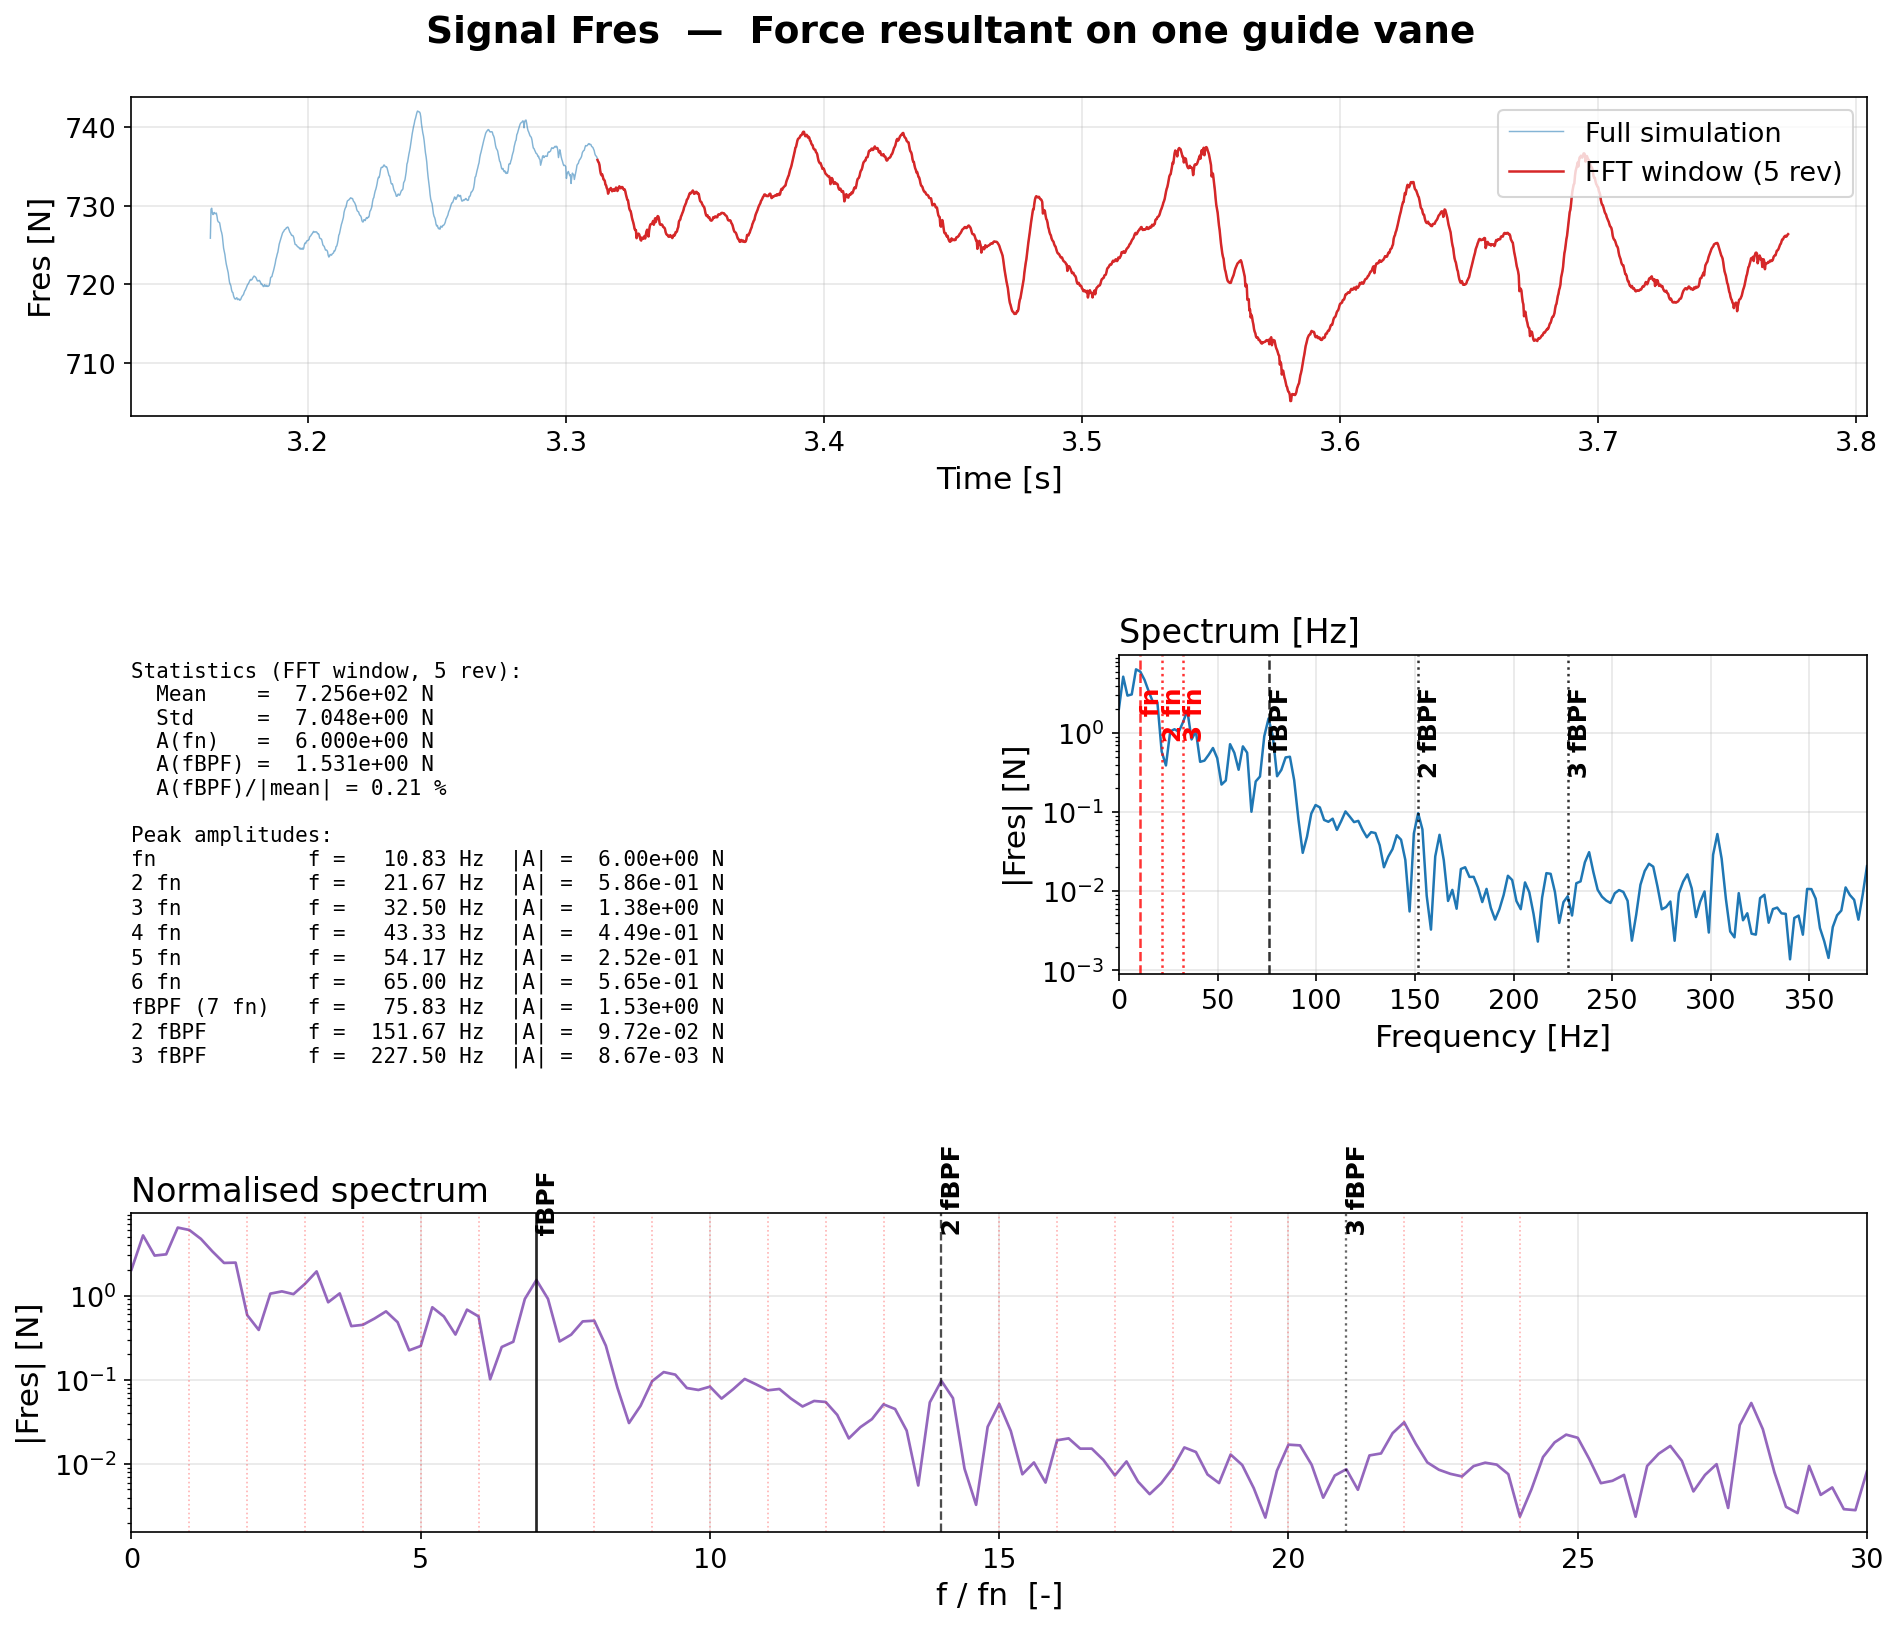
\includegraphics[width=0.99\linewidth]{Figures/FFT/signal_Fres.png}
\caption{$F_{\mathrm{res}}$ — Resultant force on one guide vane.}
\end{figure}

\begin{figure}[H]\centering
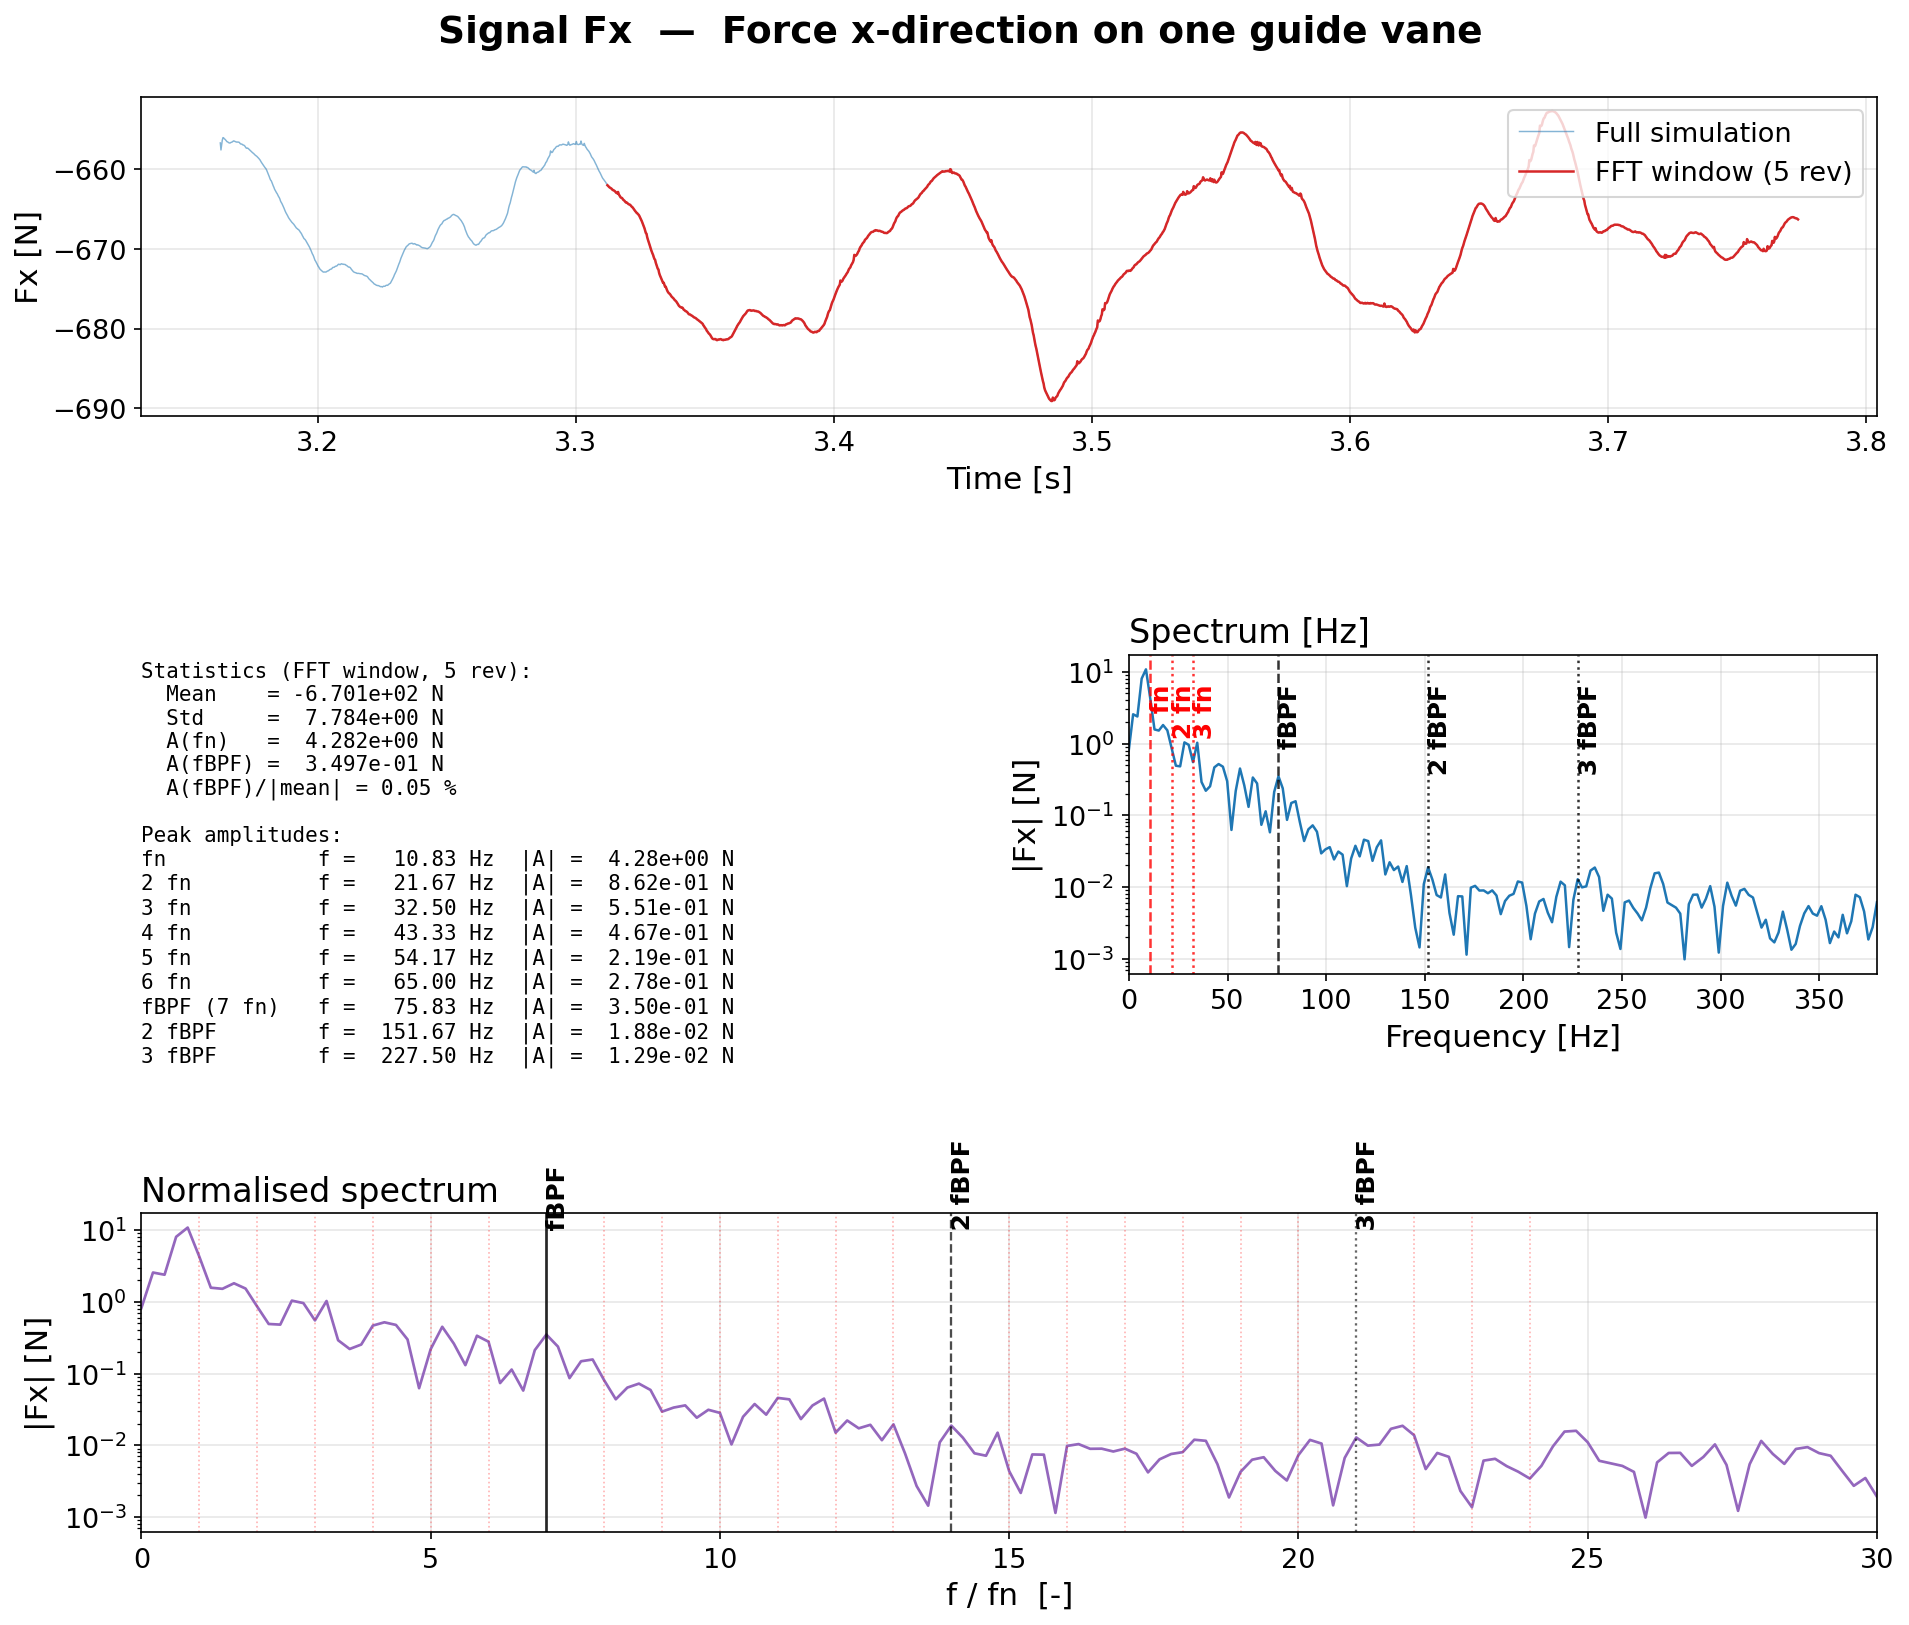
\includegraphics[width=0.99\linewidth]{Figures/FFT/signal_Fx.png}
\caption{$F_x$ — Force $x$-direction on one guide vane.}
\end{figure}

\begin{figure}[H]\centering
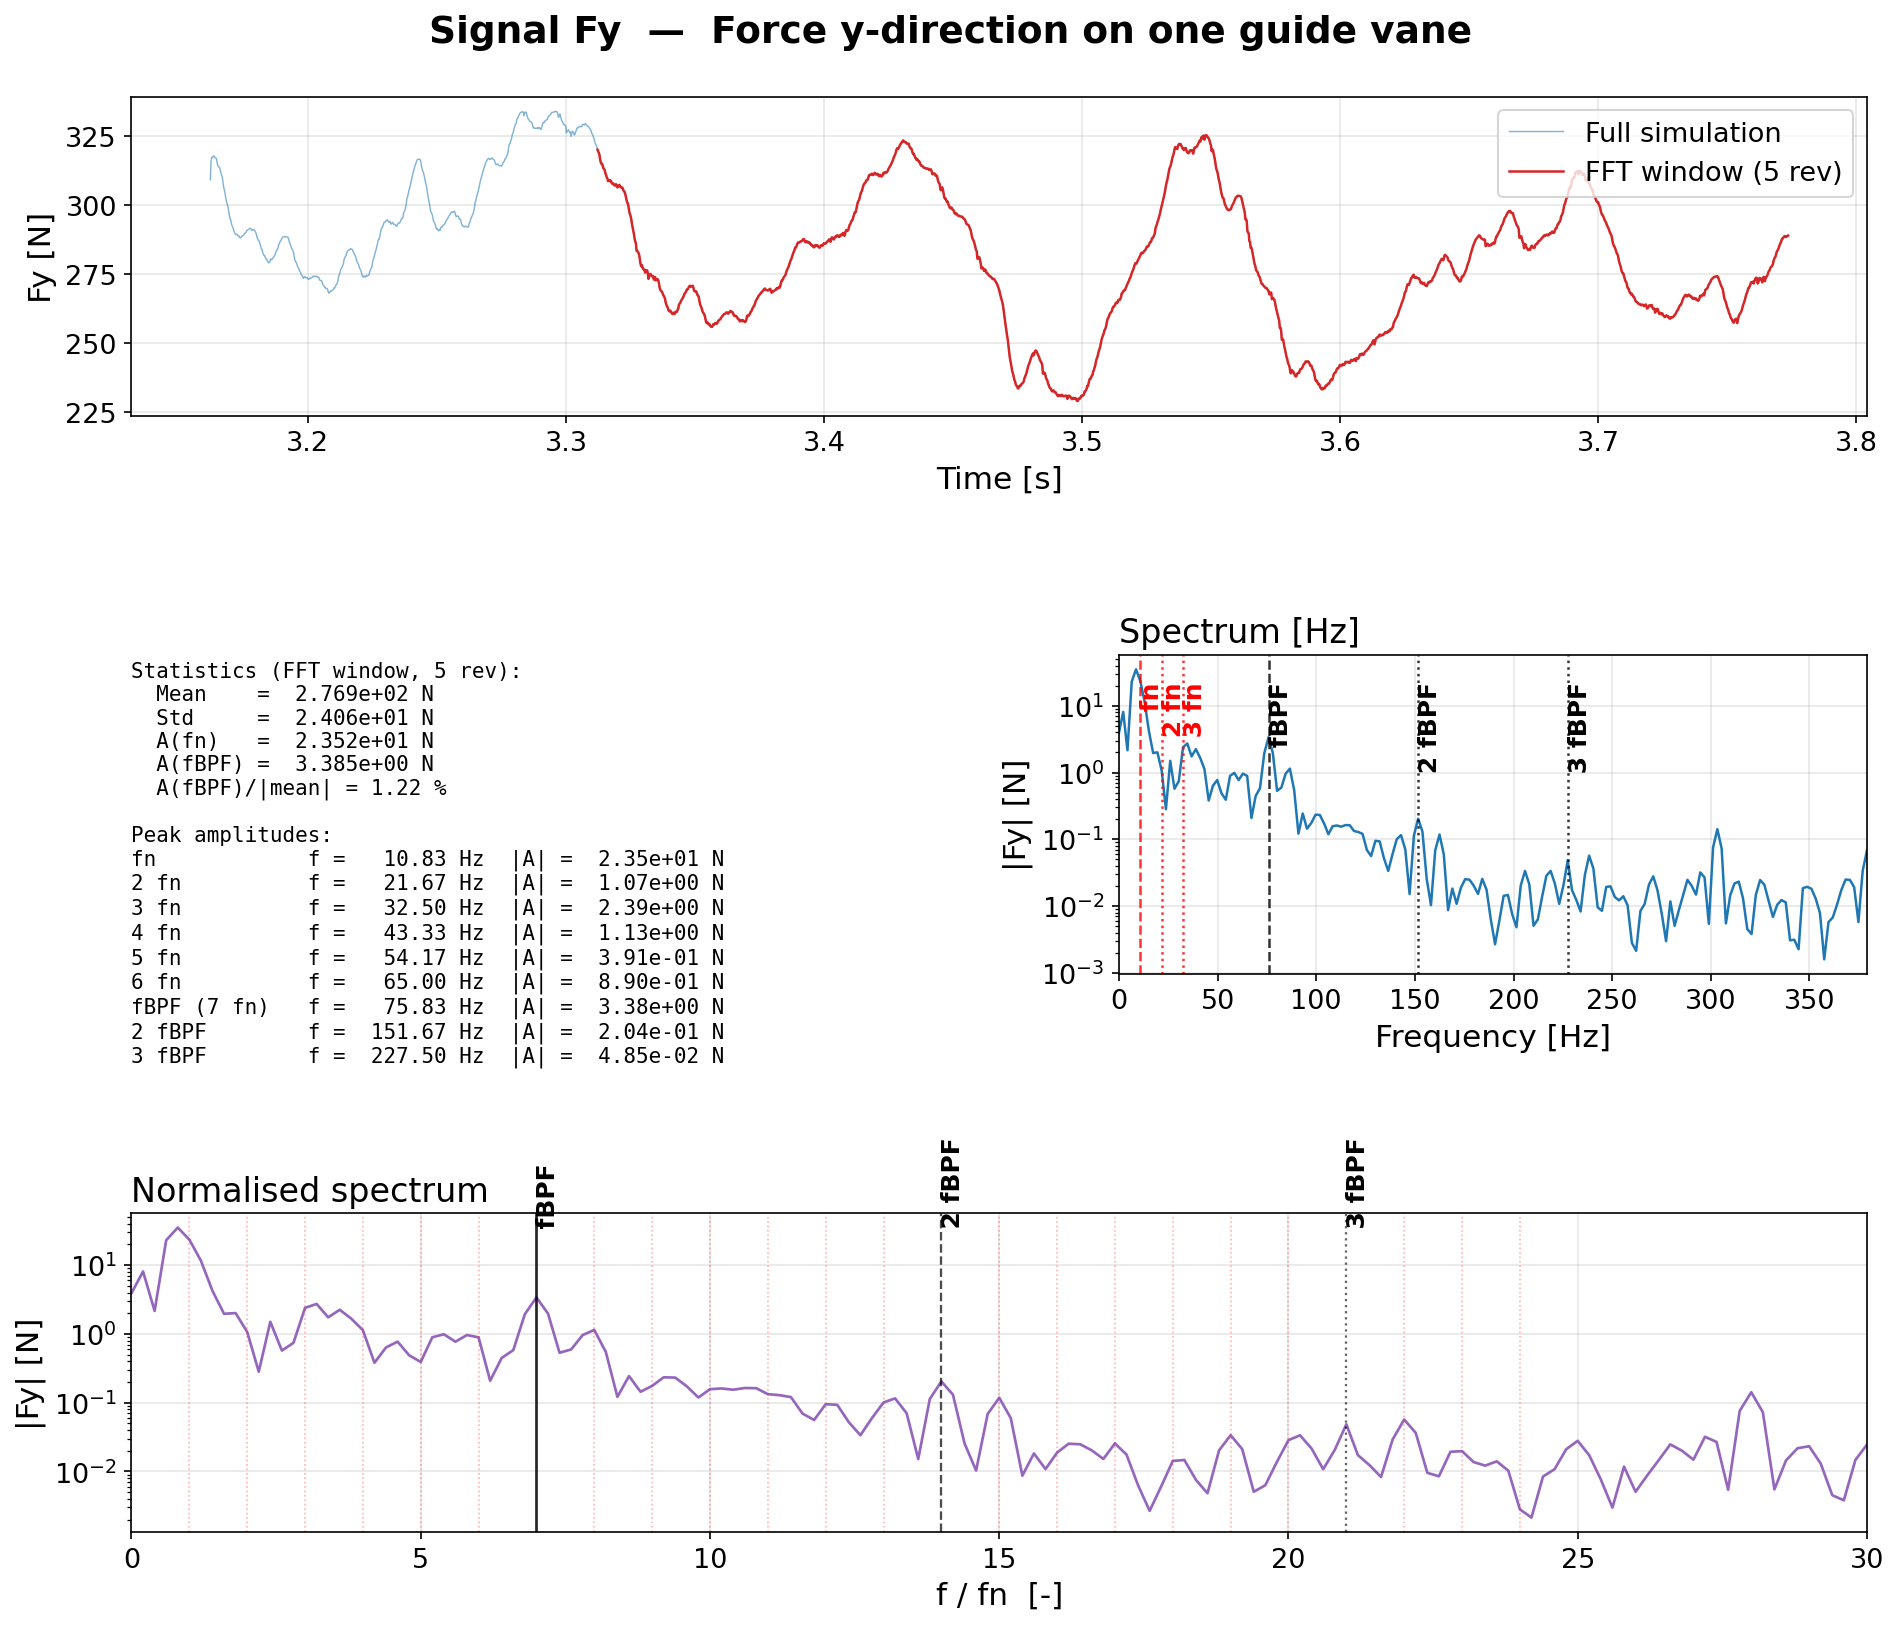
\includegraphics[width=0.99\linewidth]{Figures/FFT/signal_Fy.png}
\caption{$F_y$ — Force $y$-direction on one guide vane.}
\end{figure}

\begin{figure}[H]\centering
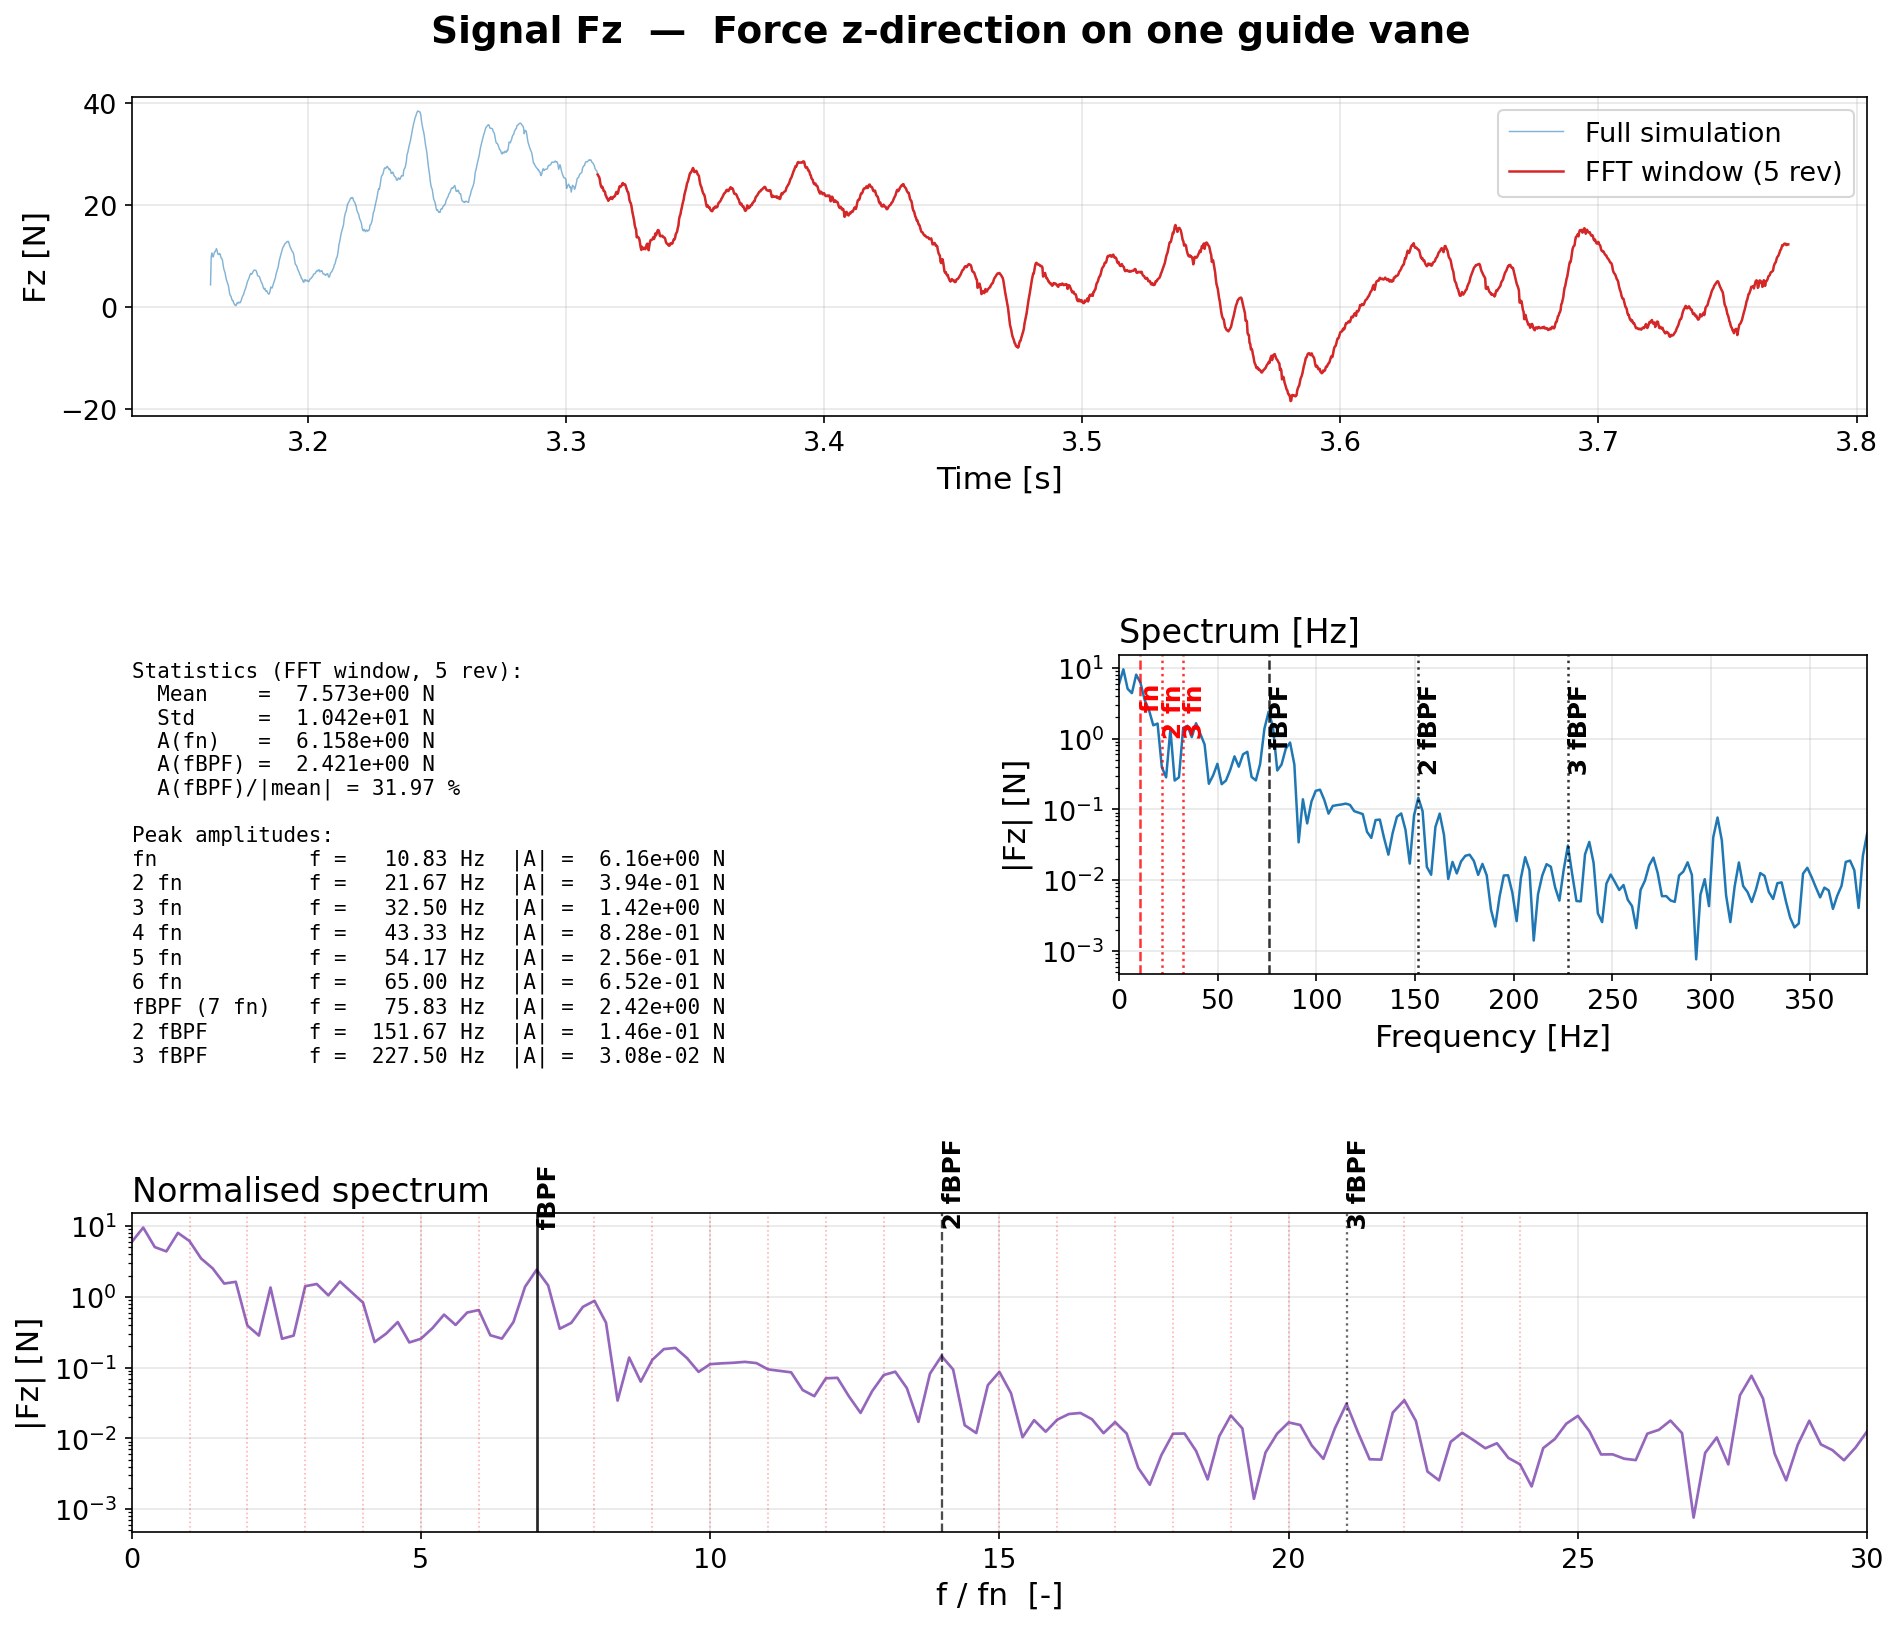
\includegraphics[width=0.99\linewidth]{Figures/FFT/signal_Fz.png}
\caption{$F_z$ — Force $z$-direction (axial) on one guide vane.}
\end{figure}

% ----- Group B: torque -------------------------------------------

\section*{Group B — Torque on the RDT}

\begin{figure}[H]\centering
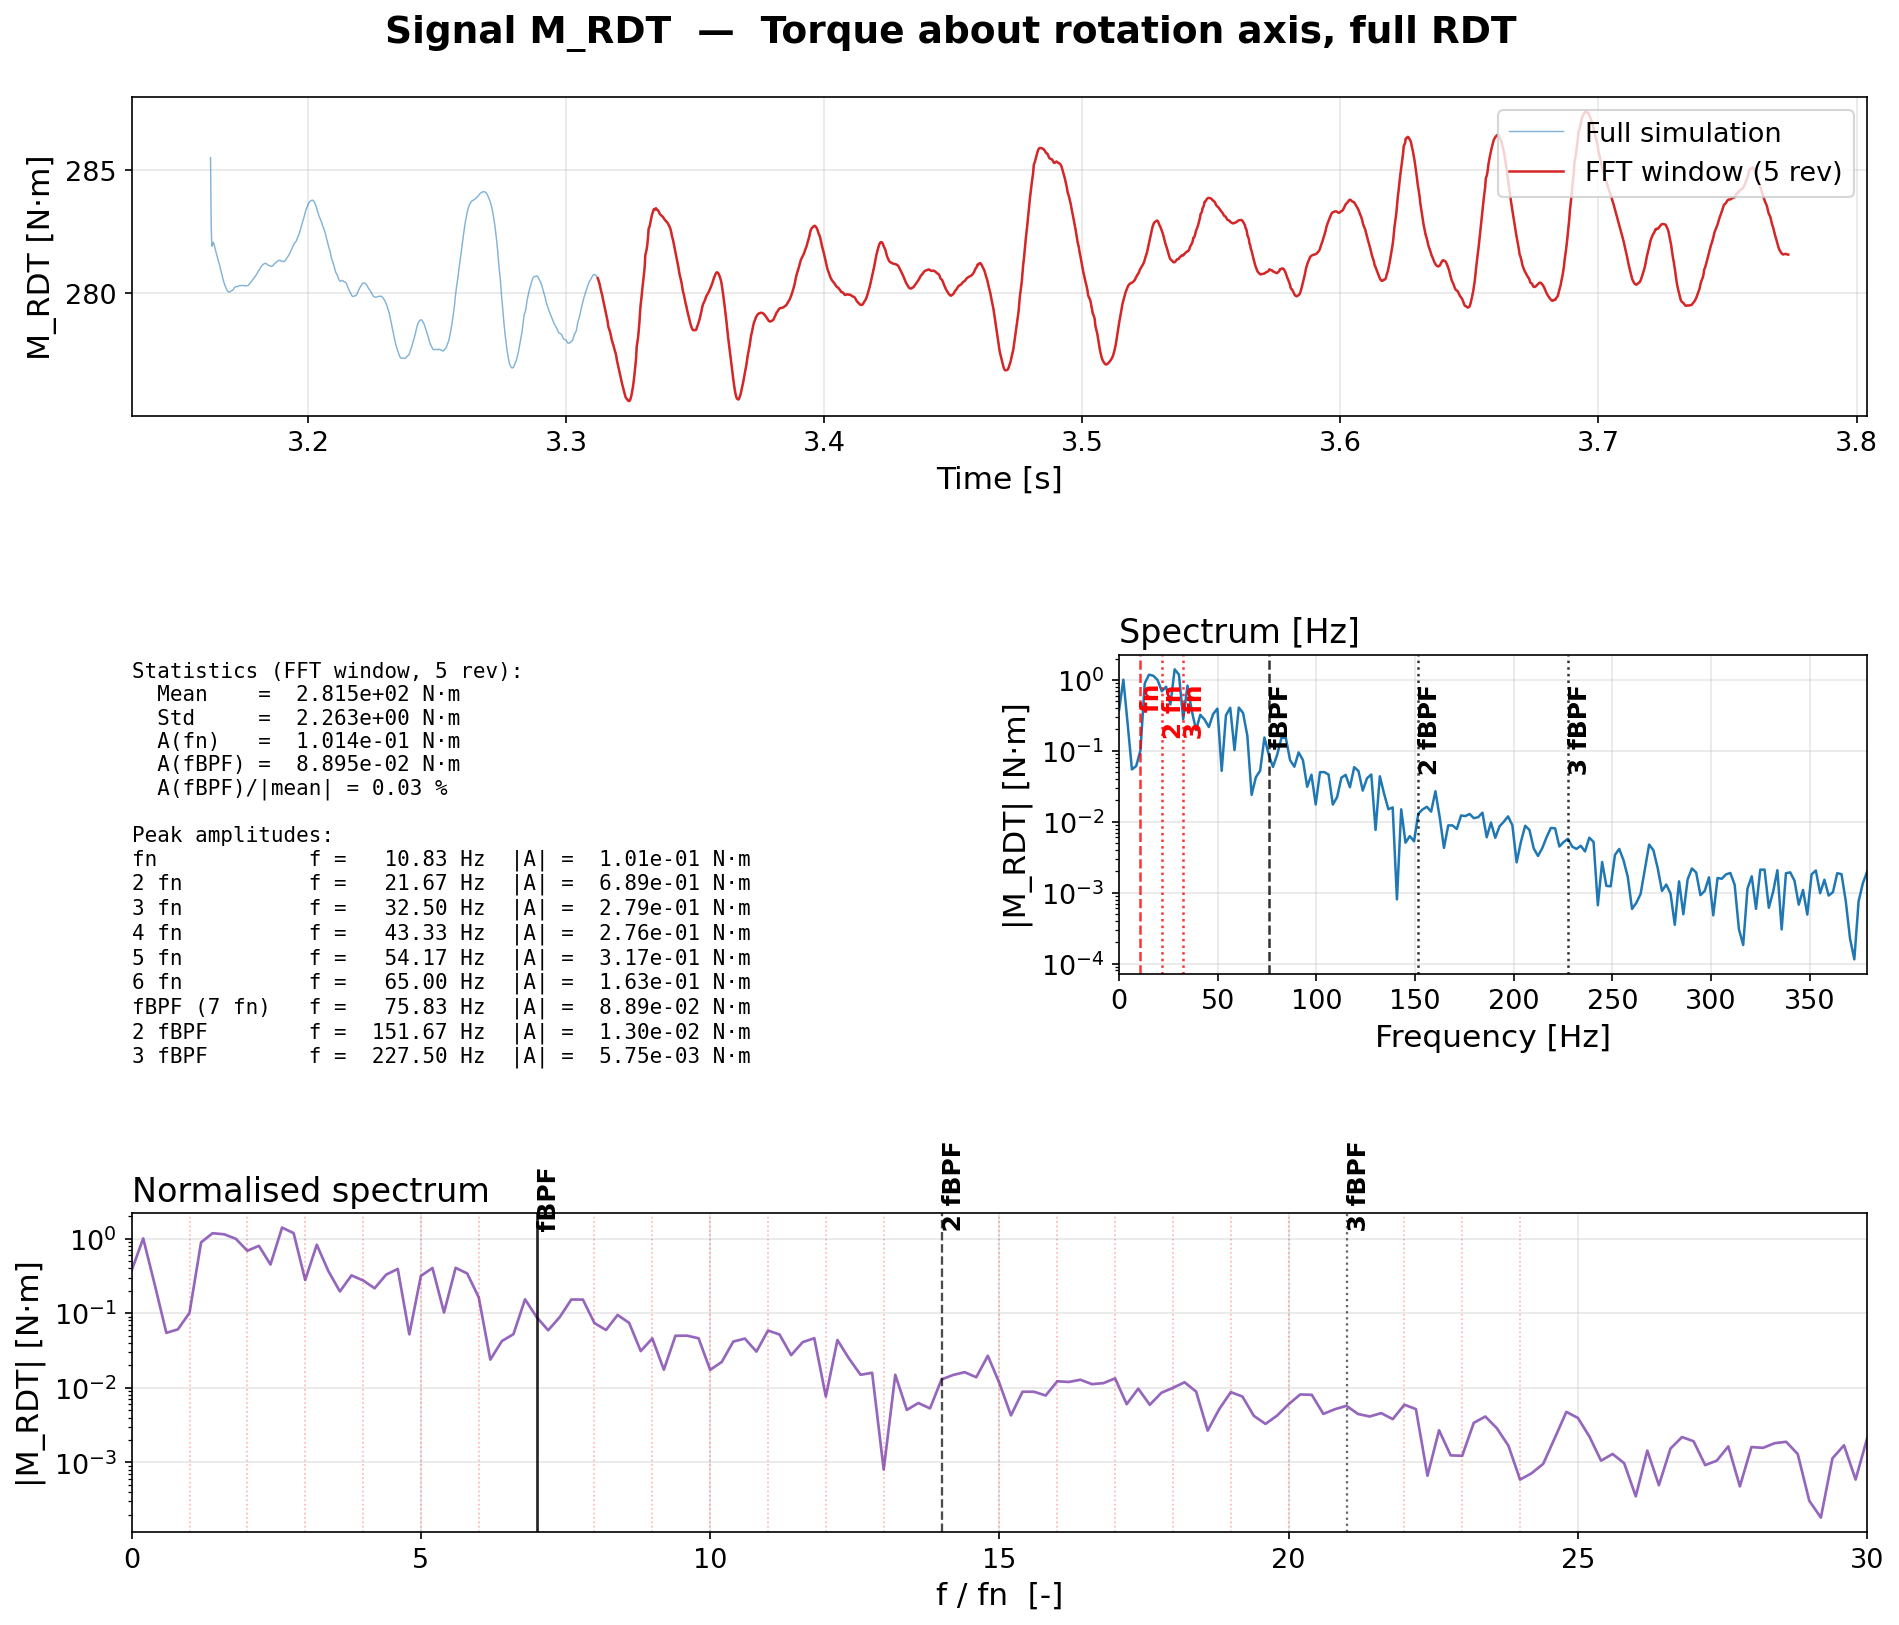
\includegraphics[width=0.99\linewidth]{Figures/FFT/signal_M_RDT.png}
\caption{$M_{\mathrm{RDT}}$ — Torque about the rotation axis,
integrated over the entire RDT blade surface.}
\end{figure}

% ----- Group C: plane-averaged pressures -------------------------

\section*{Group C — Plane-averaged pressures}

\begin{figure}[H]\centering
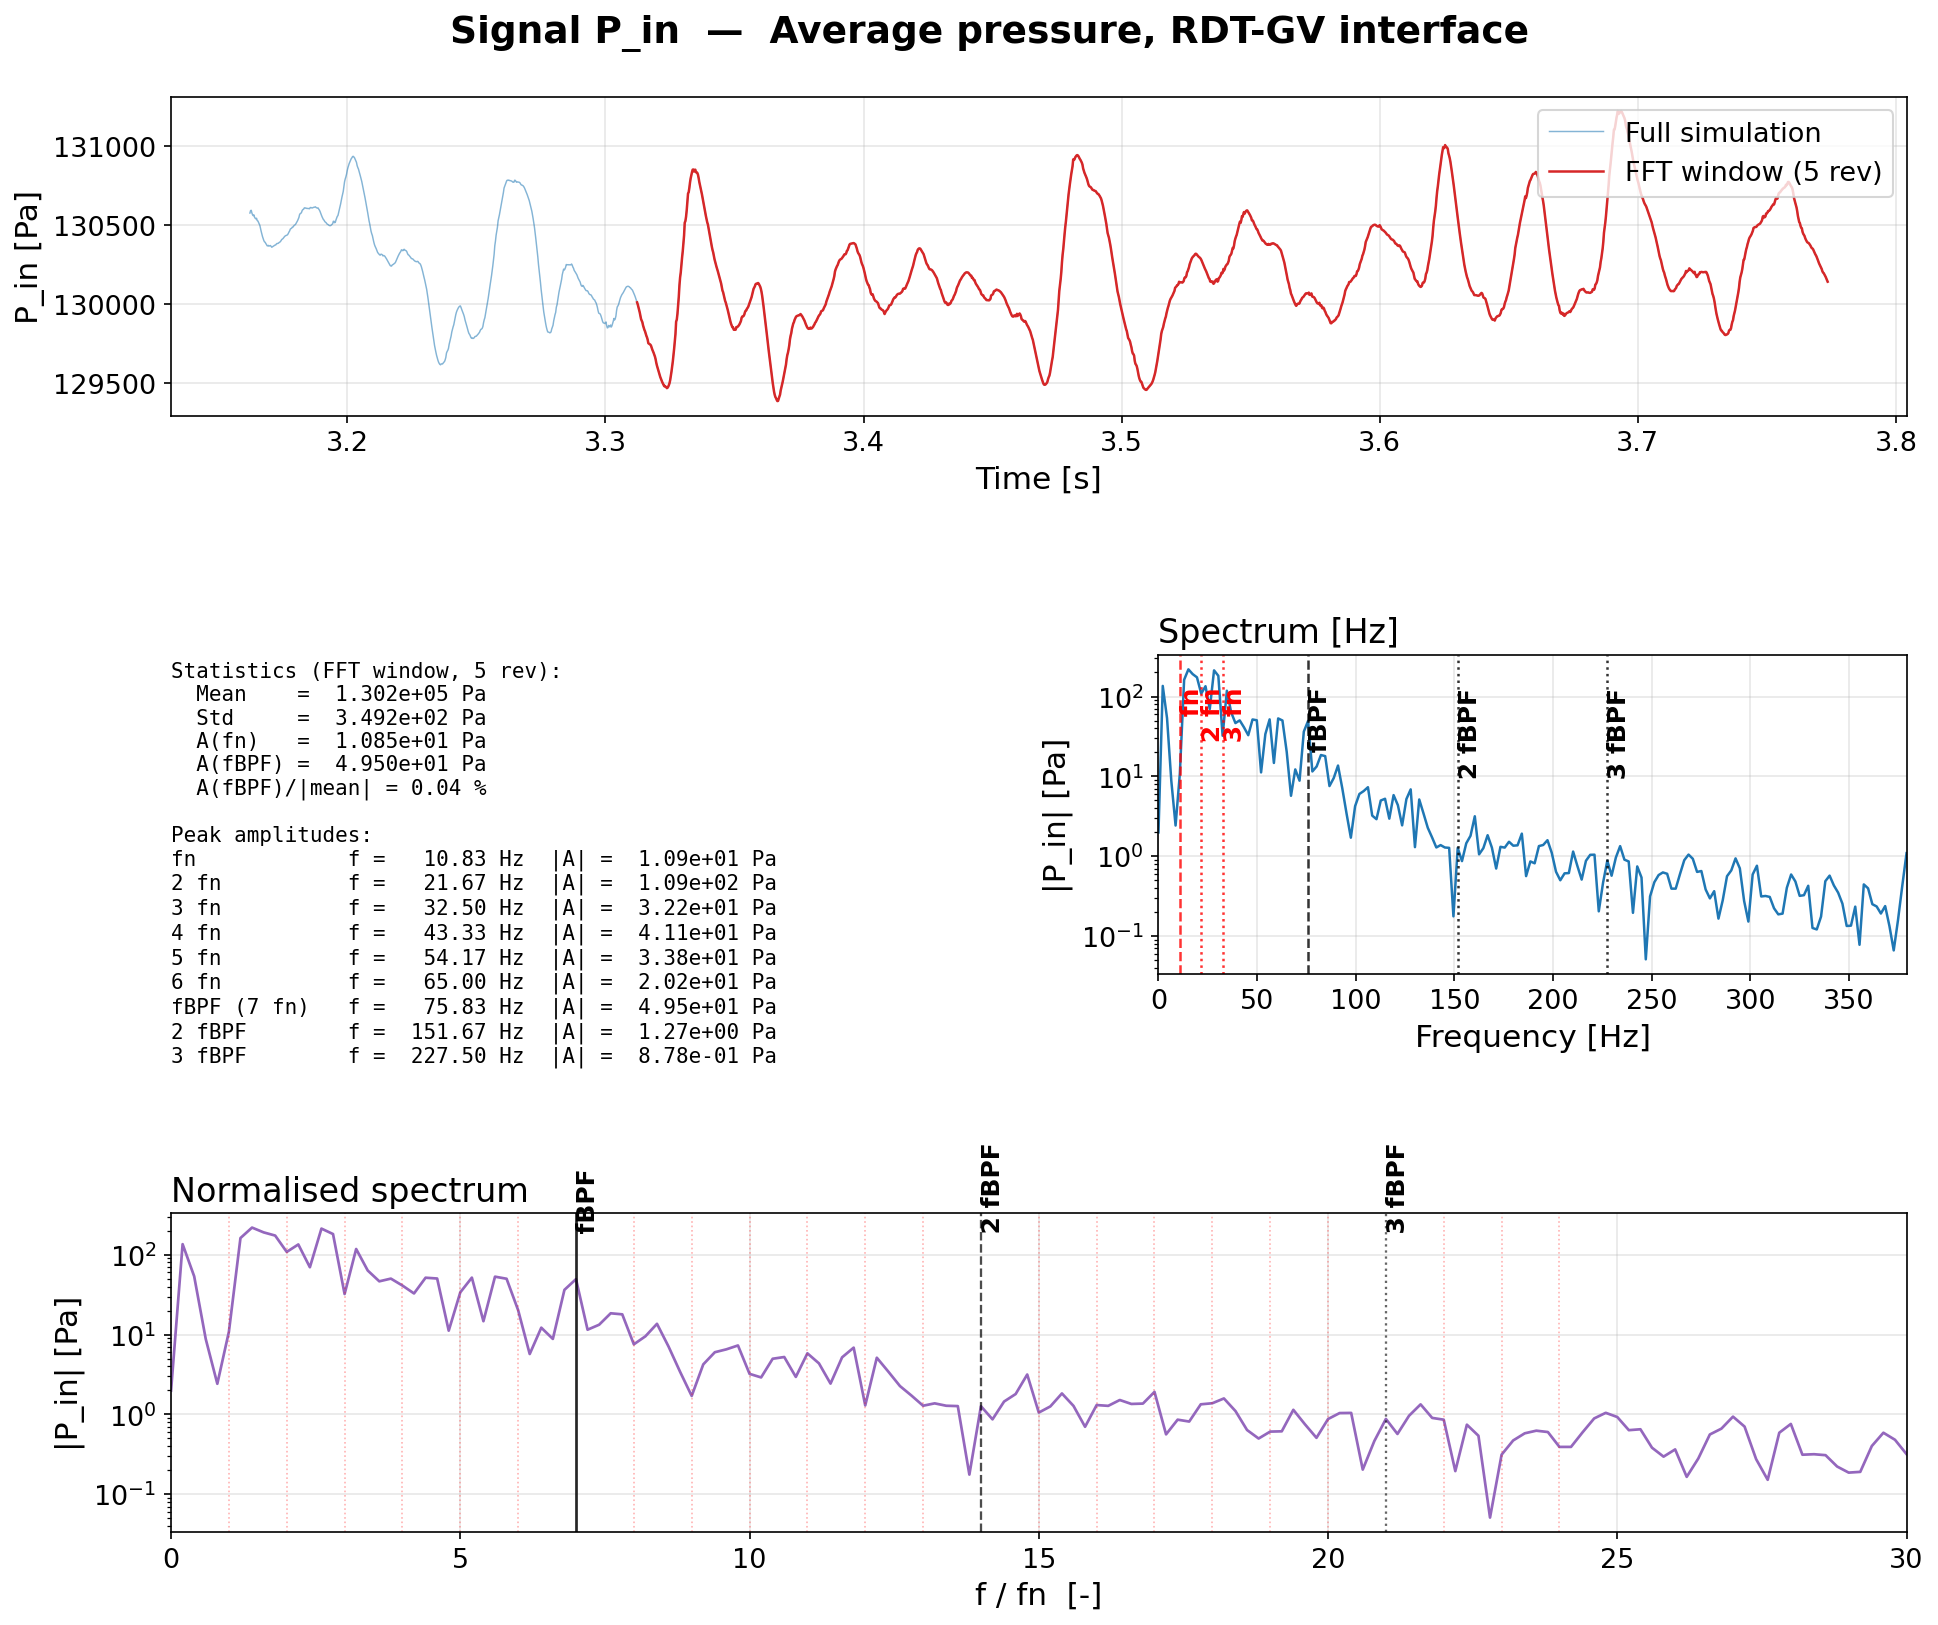
\includegraphics[width=0.99\linewidth]{Figures/FFT/signal_P_in.png}
\caption{$P_{\mathrm{in}}$ — Mass-flow-averaged pressure at the
RDT--GV interface ($s = 0$~mm).}
\end{figure}

\begin{figure}[H]\centering
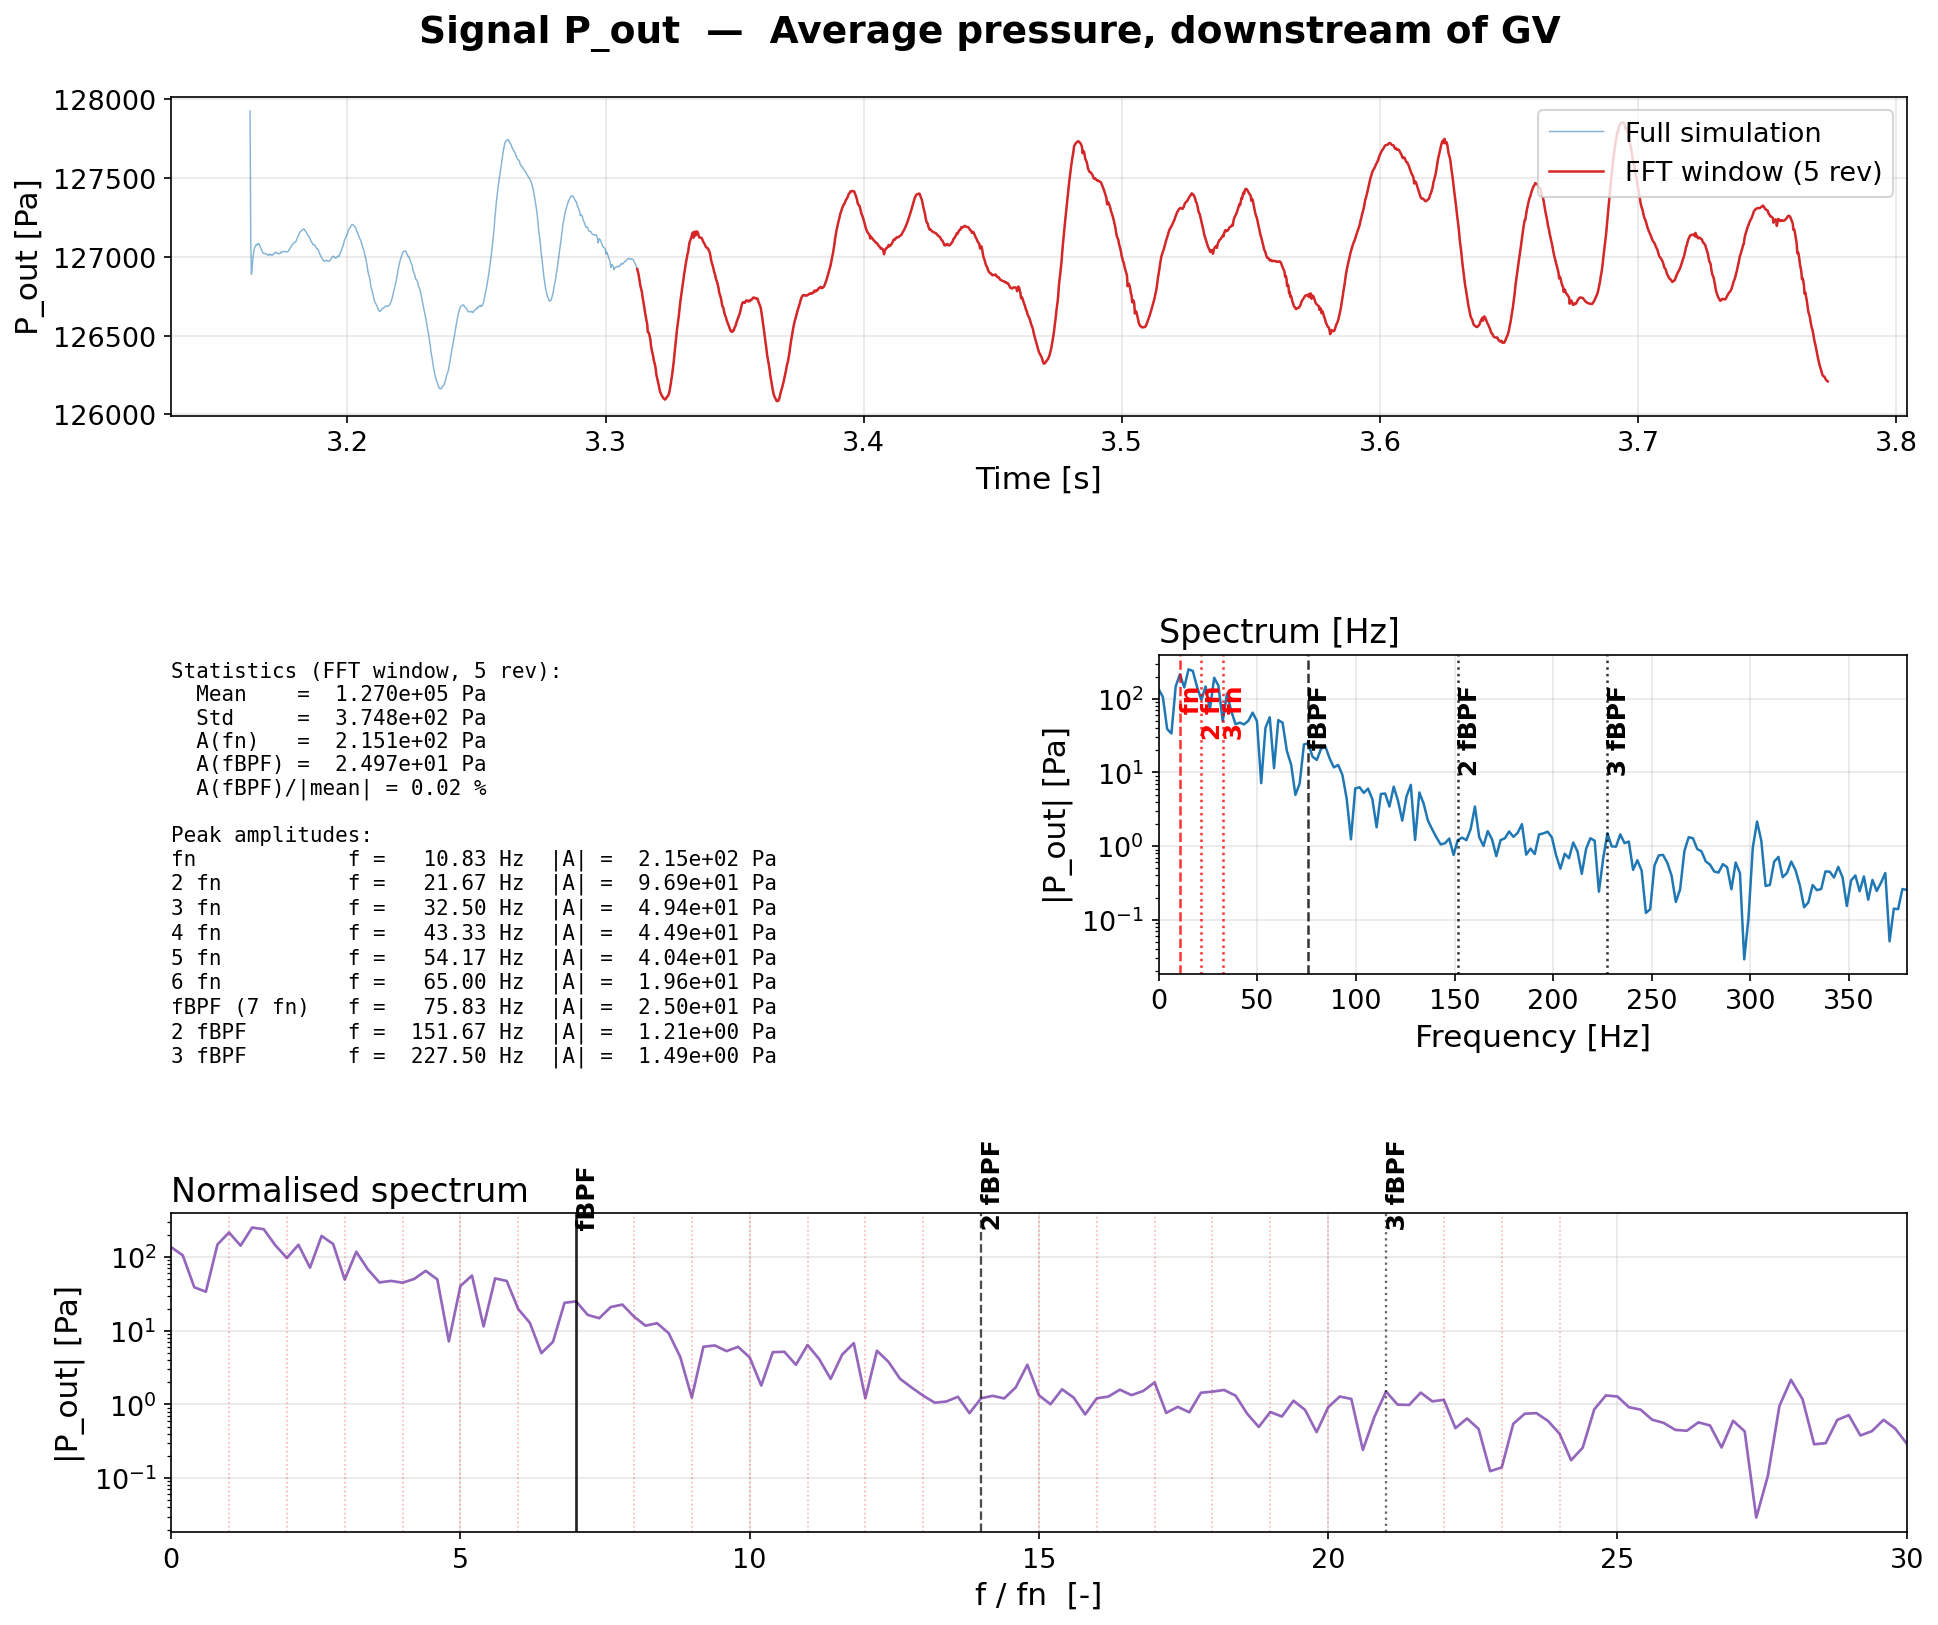
\includegraphics[width=0.99\linewidth]{Figures/FFT/signal_P_out.png}
\caption{$P_{\mathrm{out}}$ — Mass-flow-averaged pressure
downstream of the GV row ($s = 500$~mm).}
\end{figure}

\begin{figure}[H]\centering
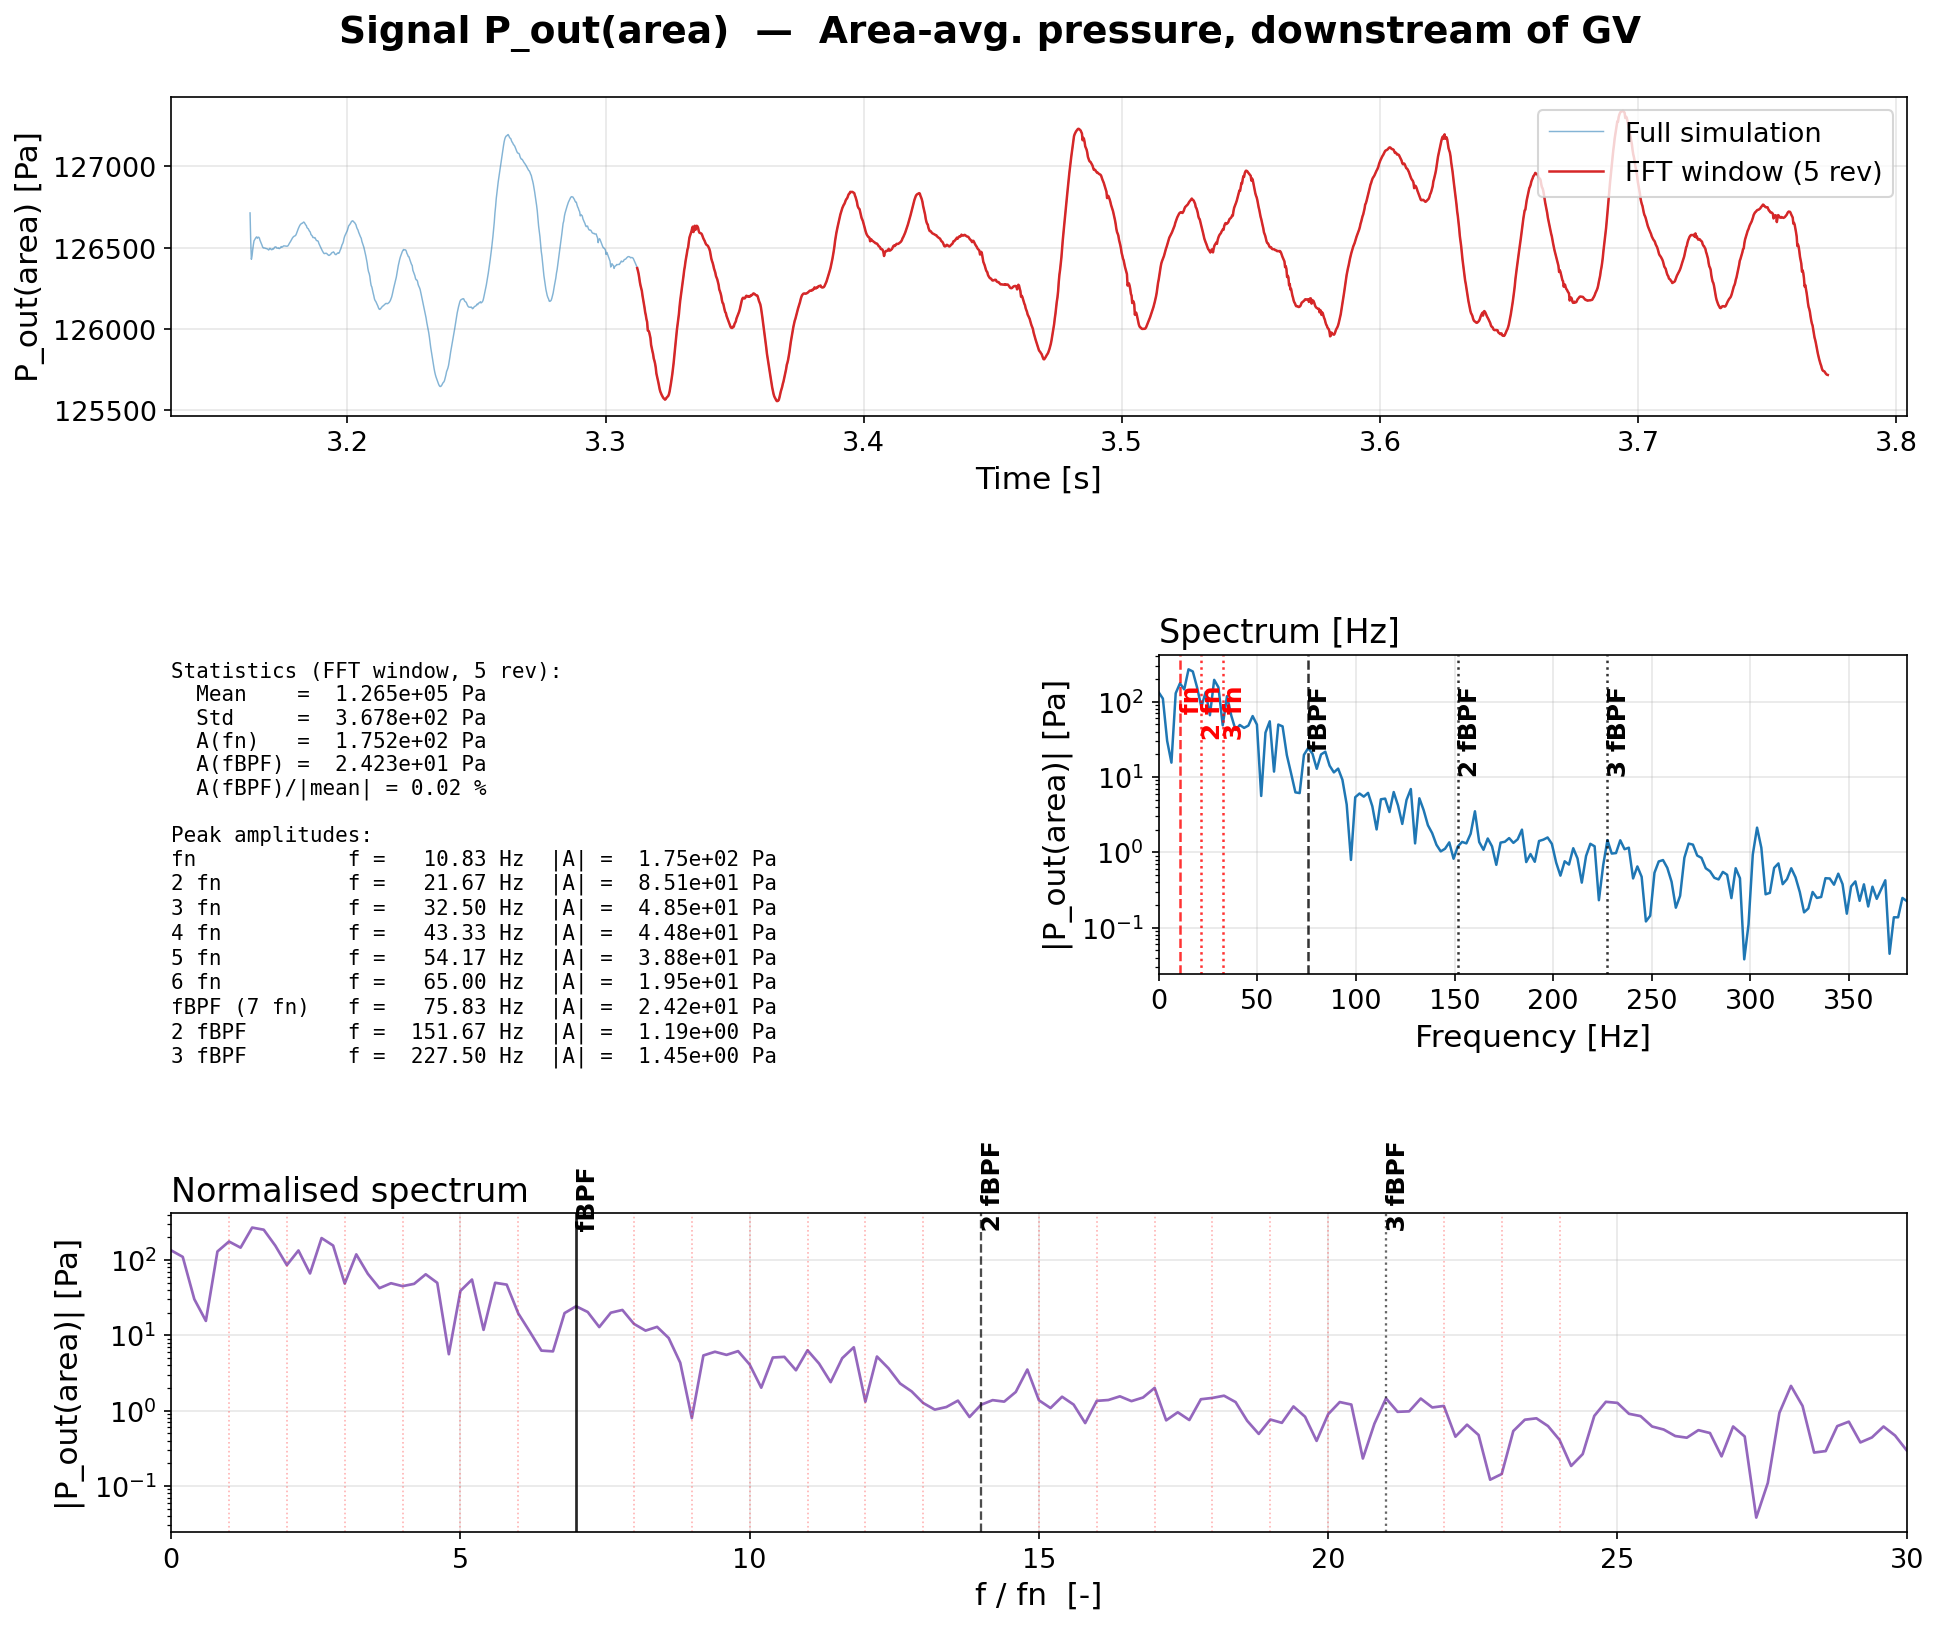
\includegraphics[width=0.99\linewidth]{Figures/FFT/signal_P_out_area.png}
\caption{$P_{\mathrm{out}}^{\,a}$ — Area-averaged pressure
downstream of the GV row (reference check only).}
\end{figure}

% ----- Group D: centre-of-pipe before bend -----------------------

\section*{Group D — Centre of pipe before the 90$^\circ$ bend}

\begin{figure}[H]\centering
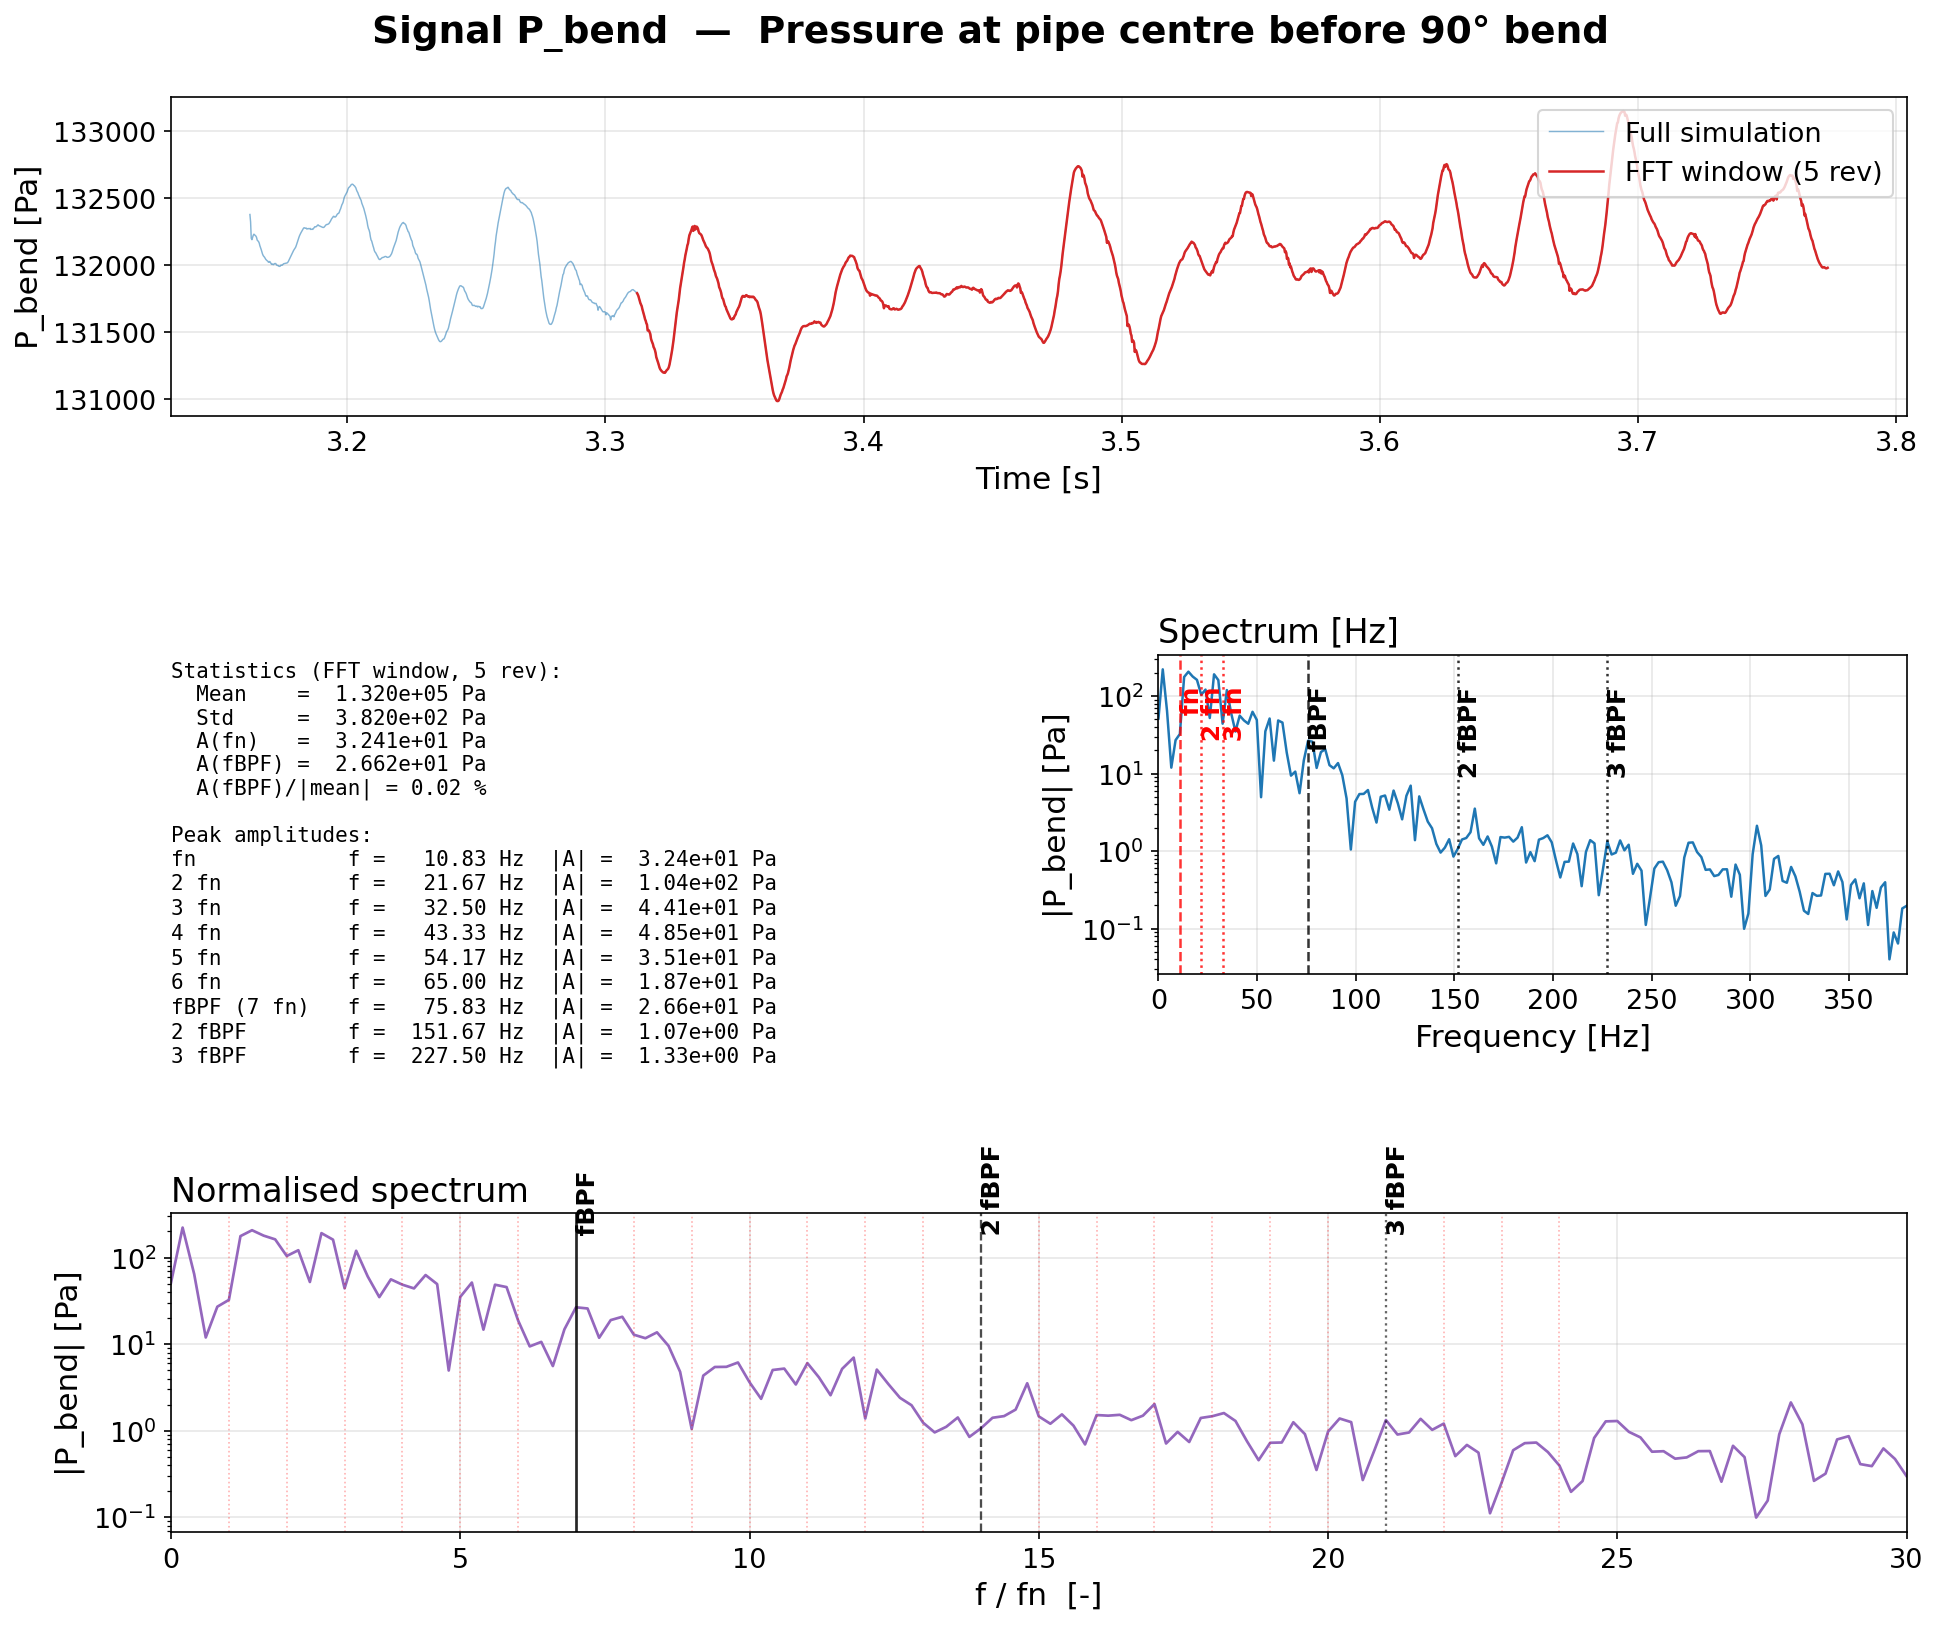
\includegraphics[width=0.99\linewidth]{Figures/FFT/signal_P_bend.png}
\caption{$P_{\mathrm{bend}}$ — Pressure at the centre of the pipe
before the 90$^\circ$ bend ($z = -2.185$~m).}
\end{figure}

% ----- Group E: wall probes along the GV passage -----------------

\section*{Group E — Wall-pressure probes along the GV passage}

\begin{figure}[H]\centering
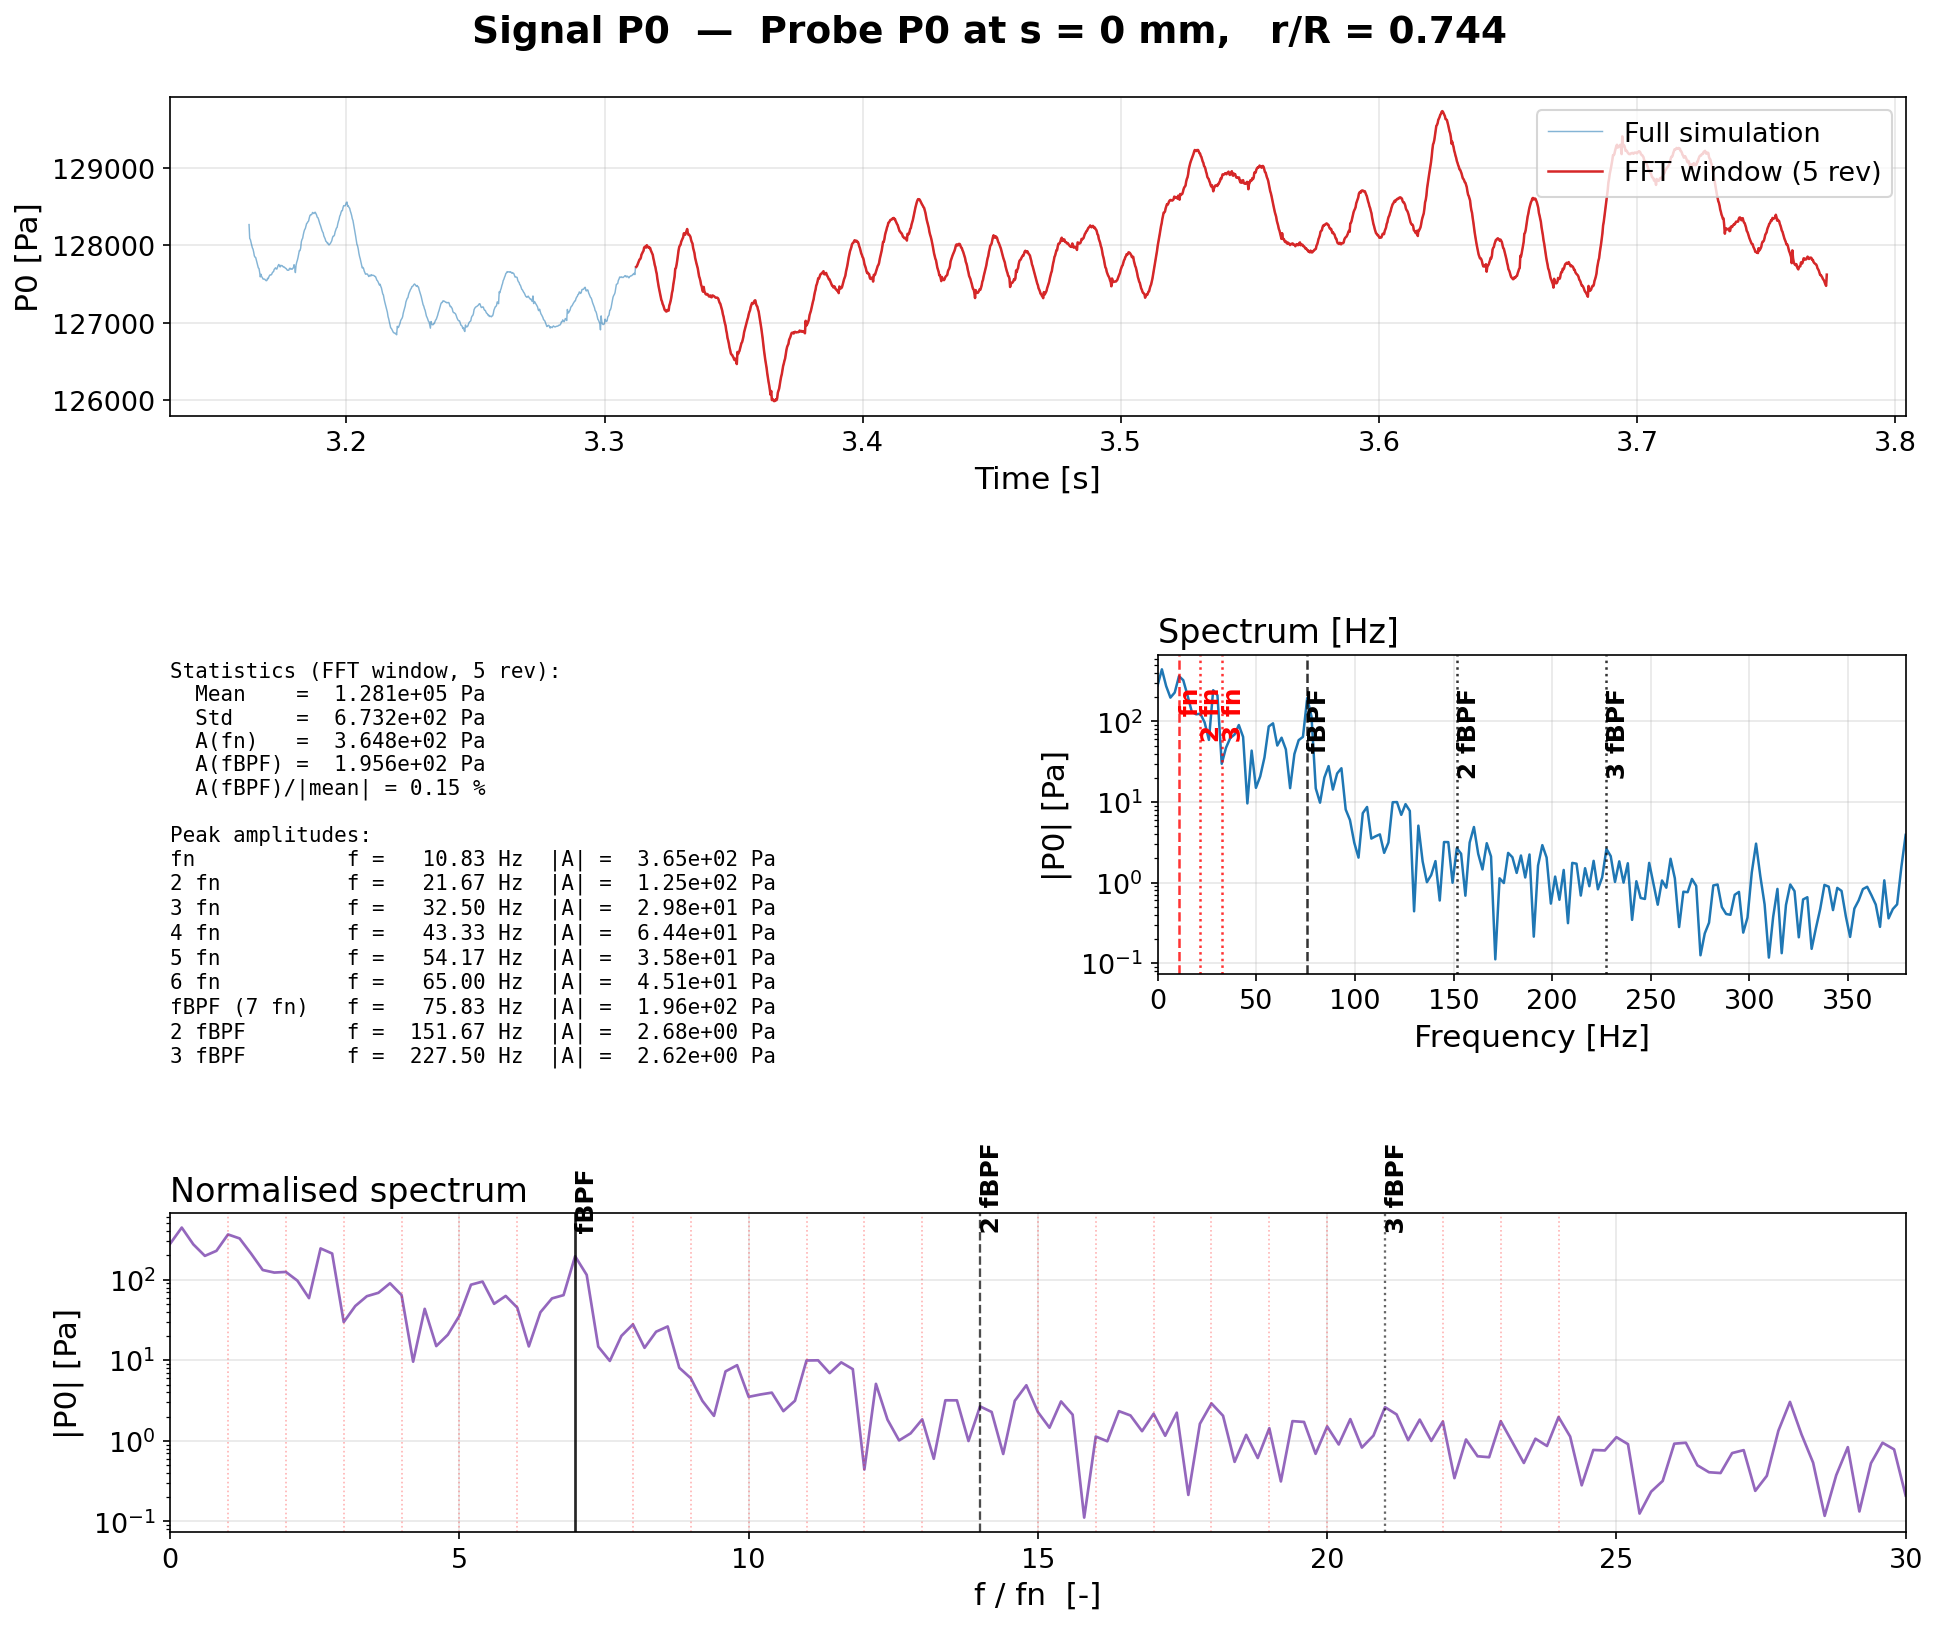
\includegraphics[width=0.99\linewidth]{Figures/FFT/signal_P0.png}
\caption{$P_0$ — Wall probe at $s = 0$~mm, $r/R = 0.744$.}
\end{figure}

\begin{figure}[H]\centering
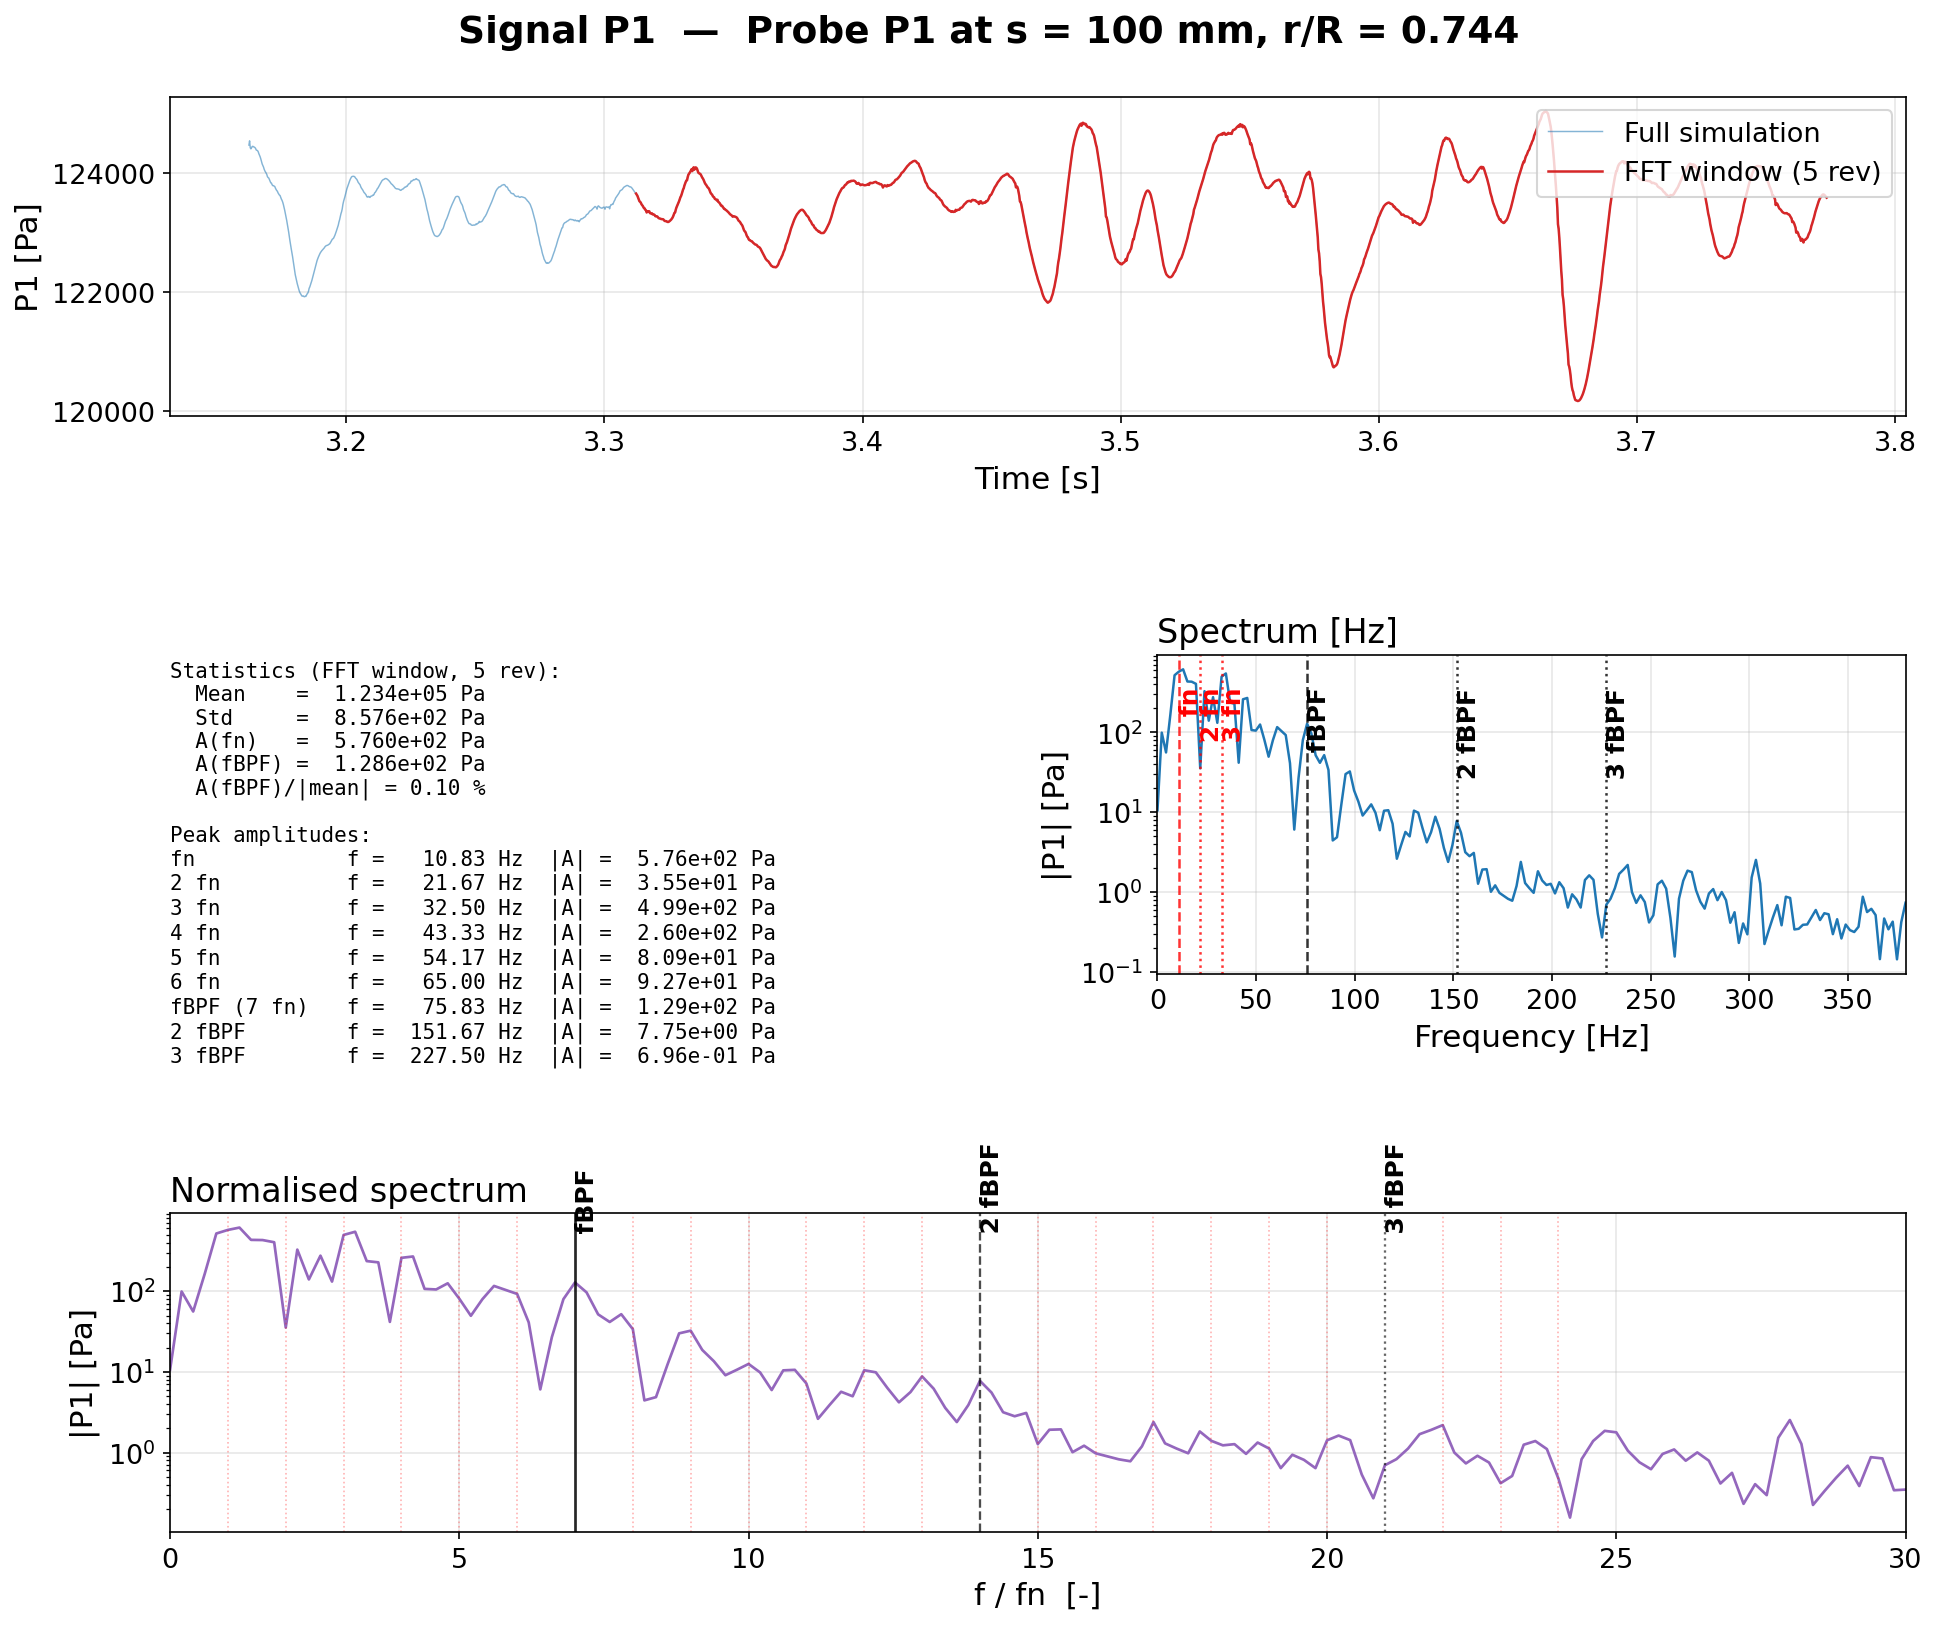
\includegraphics[width=0.99\linewidth]{Figures/FFT/signal_P1.png}
\caption{$P_1$ — Wall probe at $s = 100$~mm, $r/R = 0.744$.}
\end{figure}

\begin{figure}[H]\centering
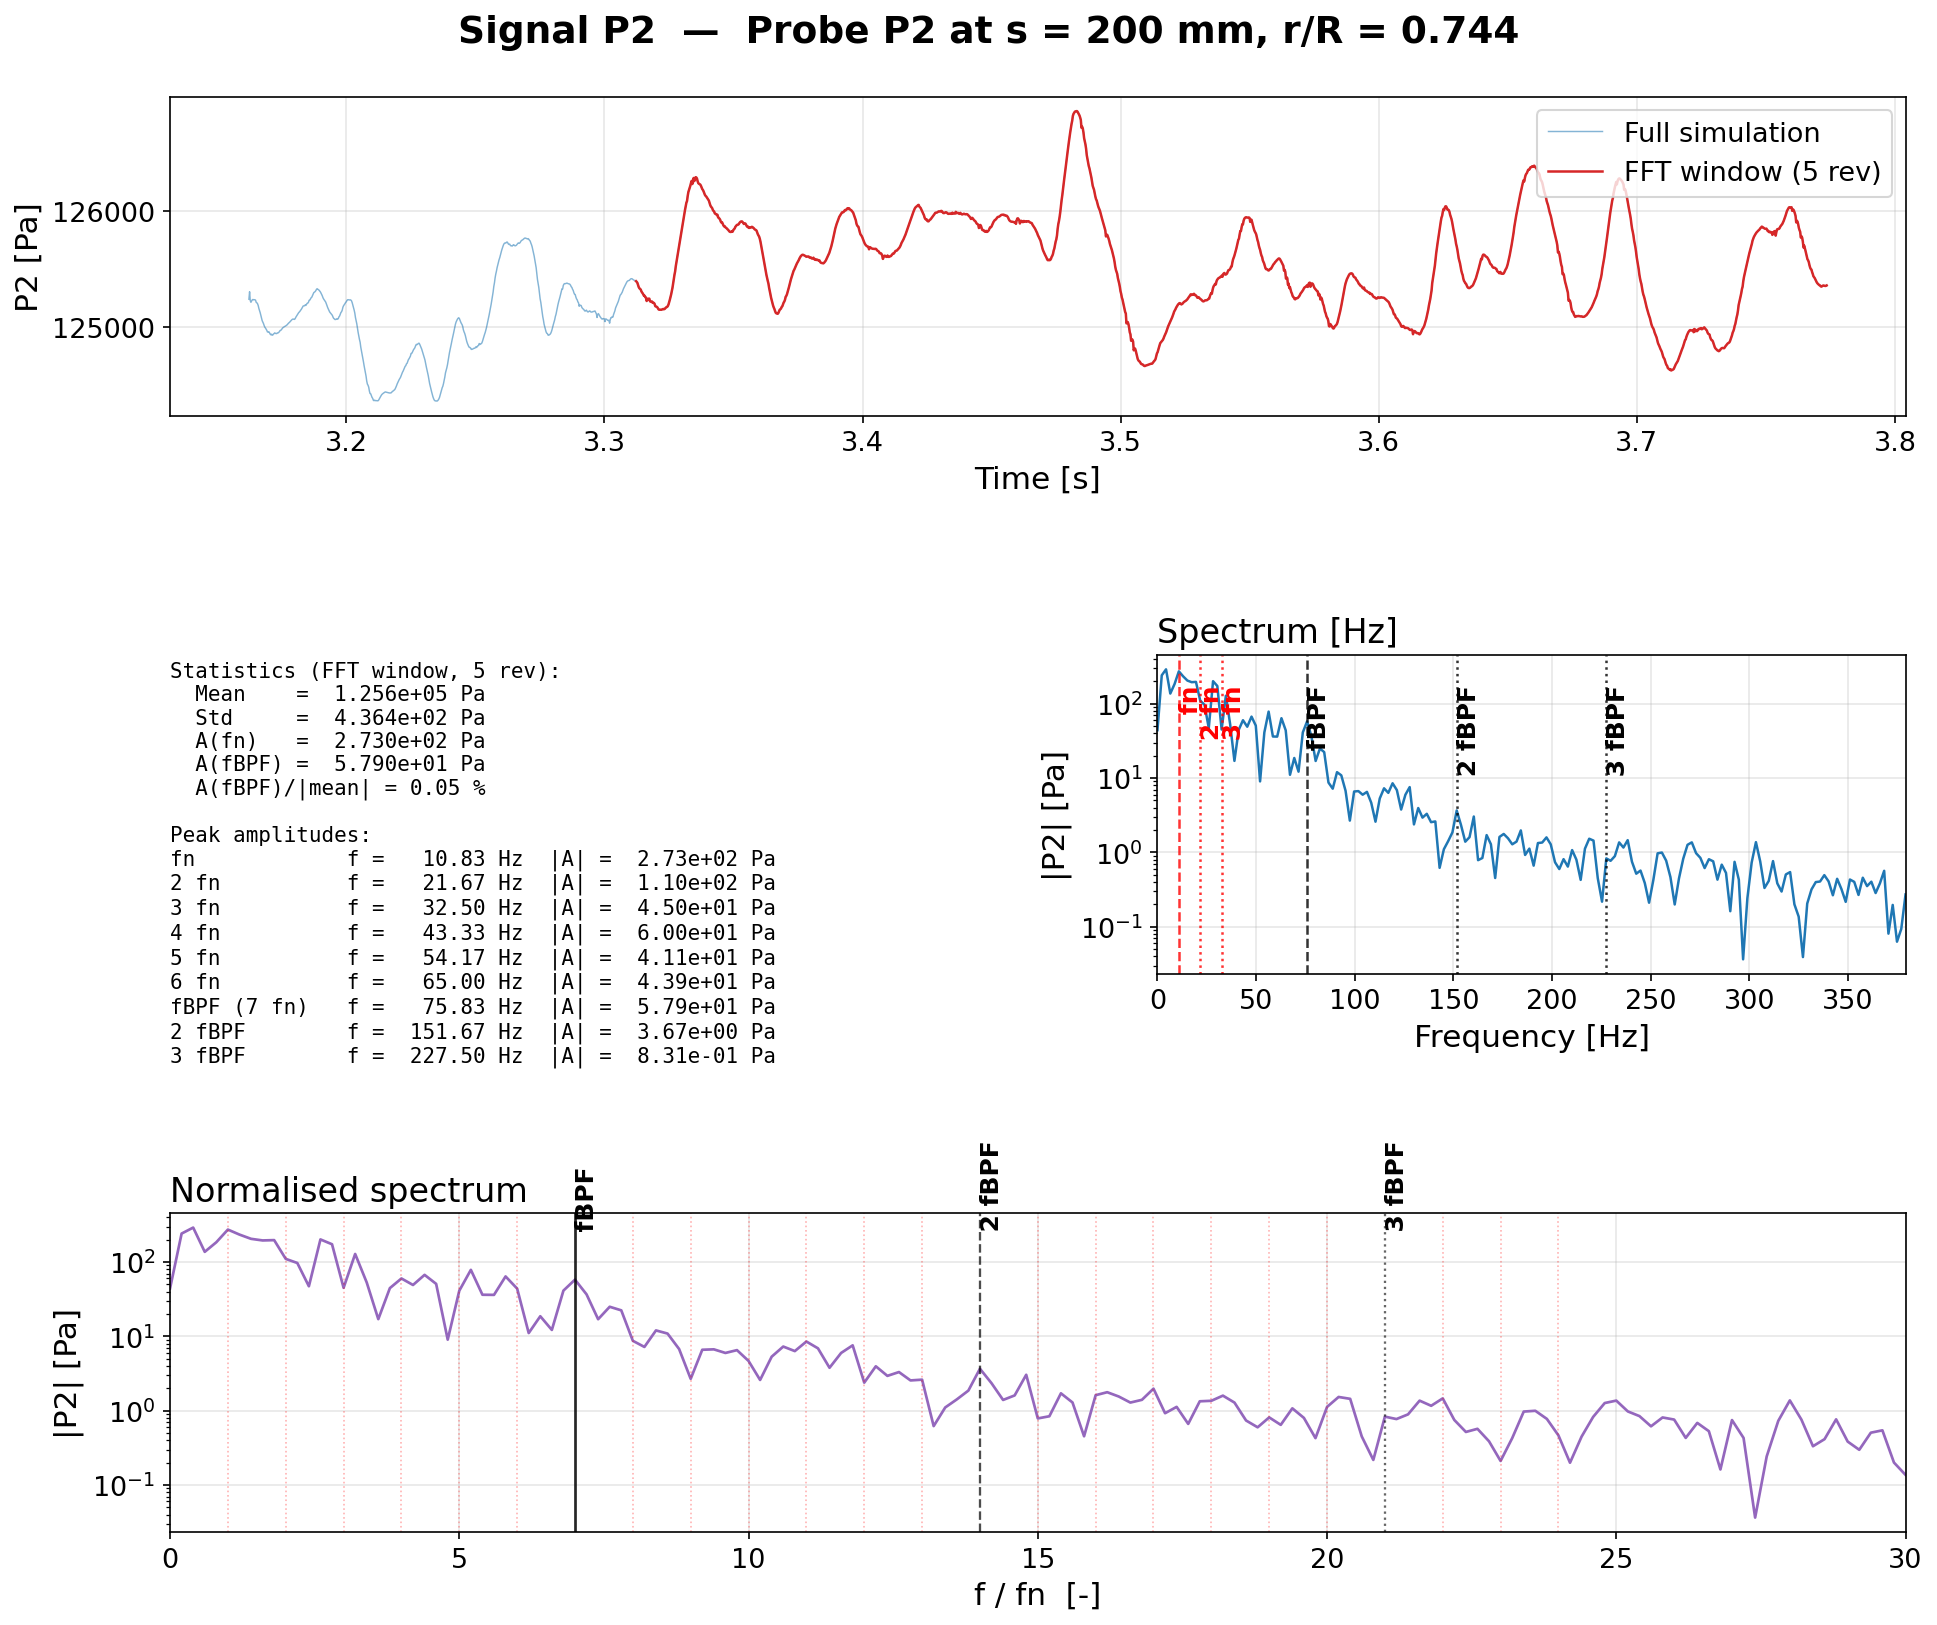
\includegraphics[width=0.99\linewidth]{Figures/FFT/signal_P2.png}
\caption{$P_2$ — Wall probe at $s = 200$~mm, $r/R = 0.744$.}
\end{figure}

\begin{figure}[H]\centering
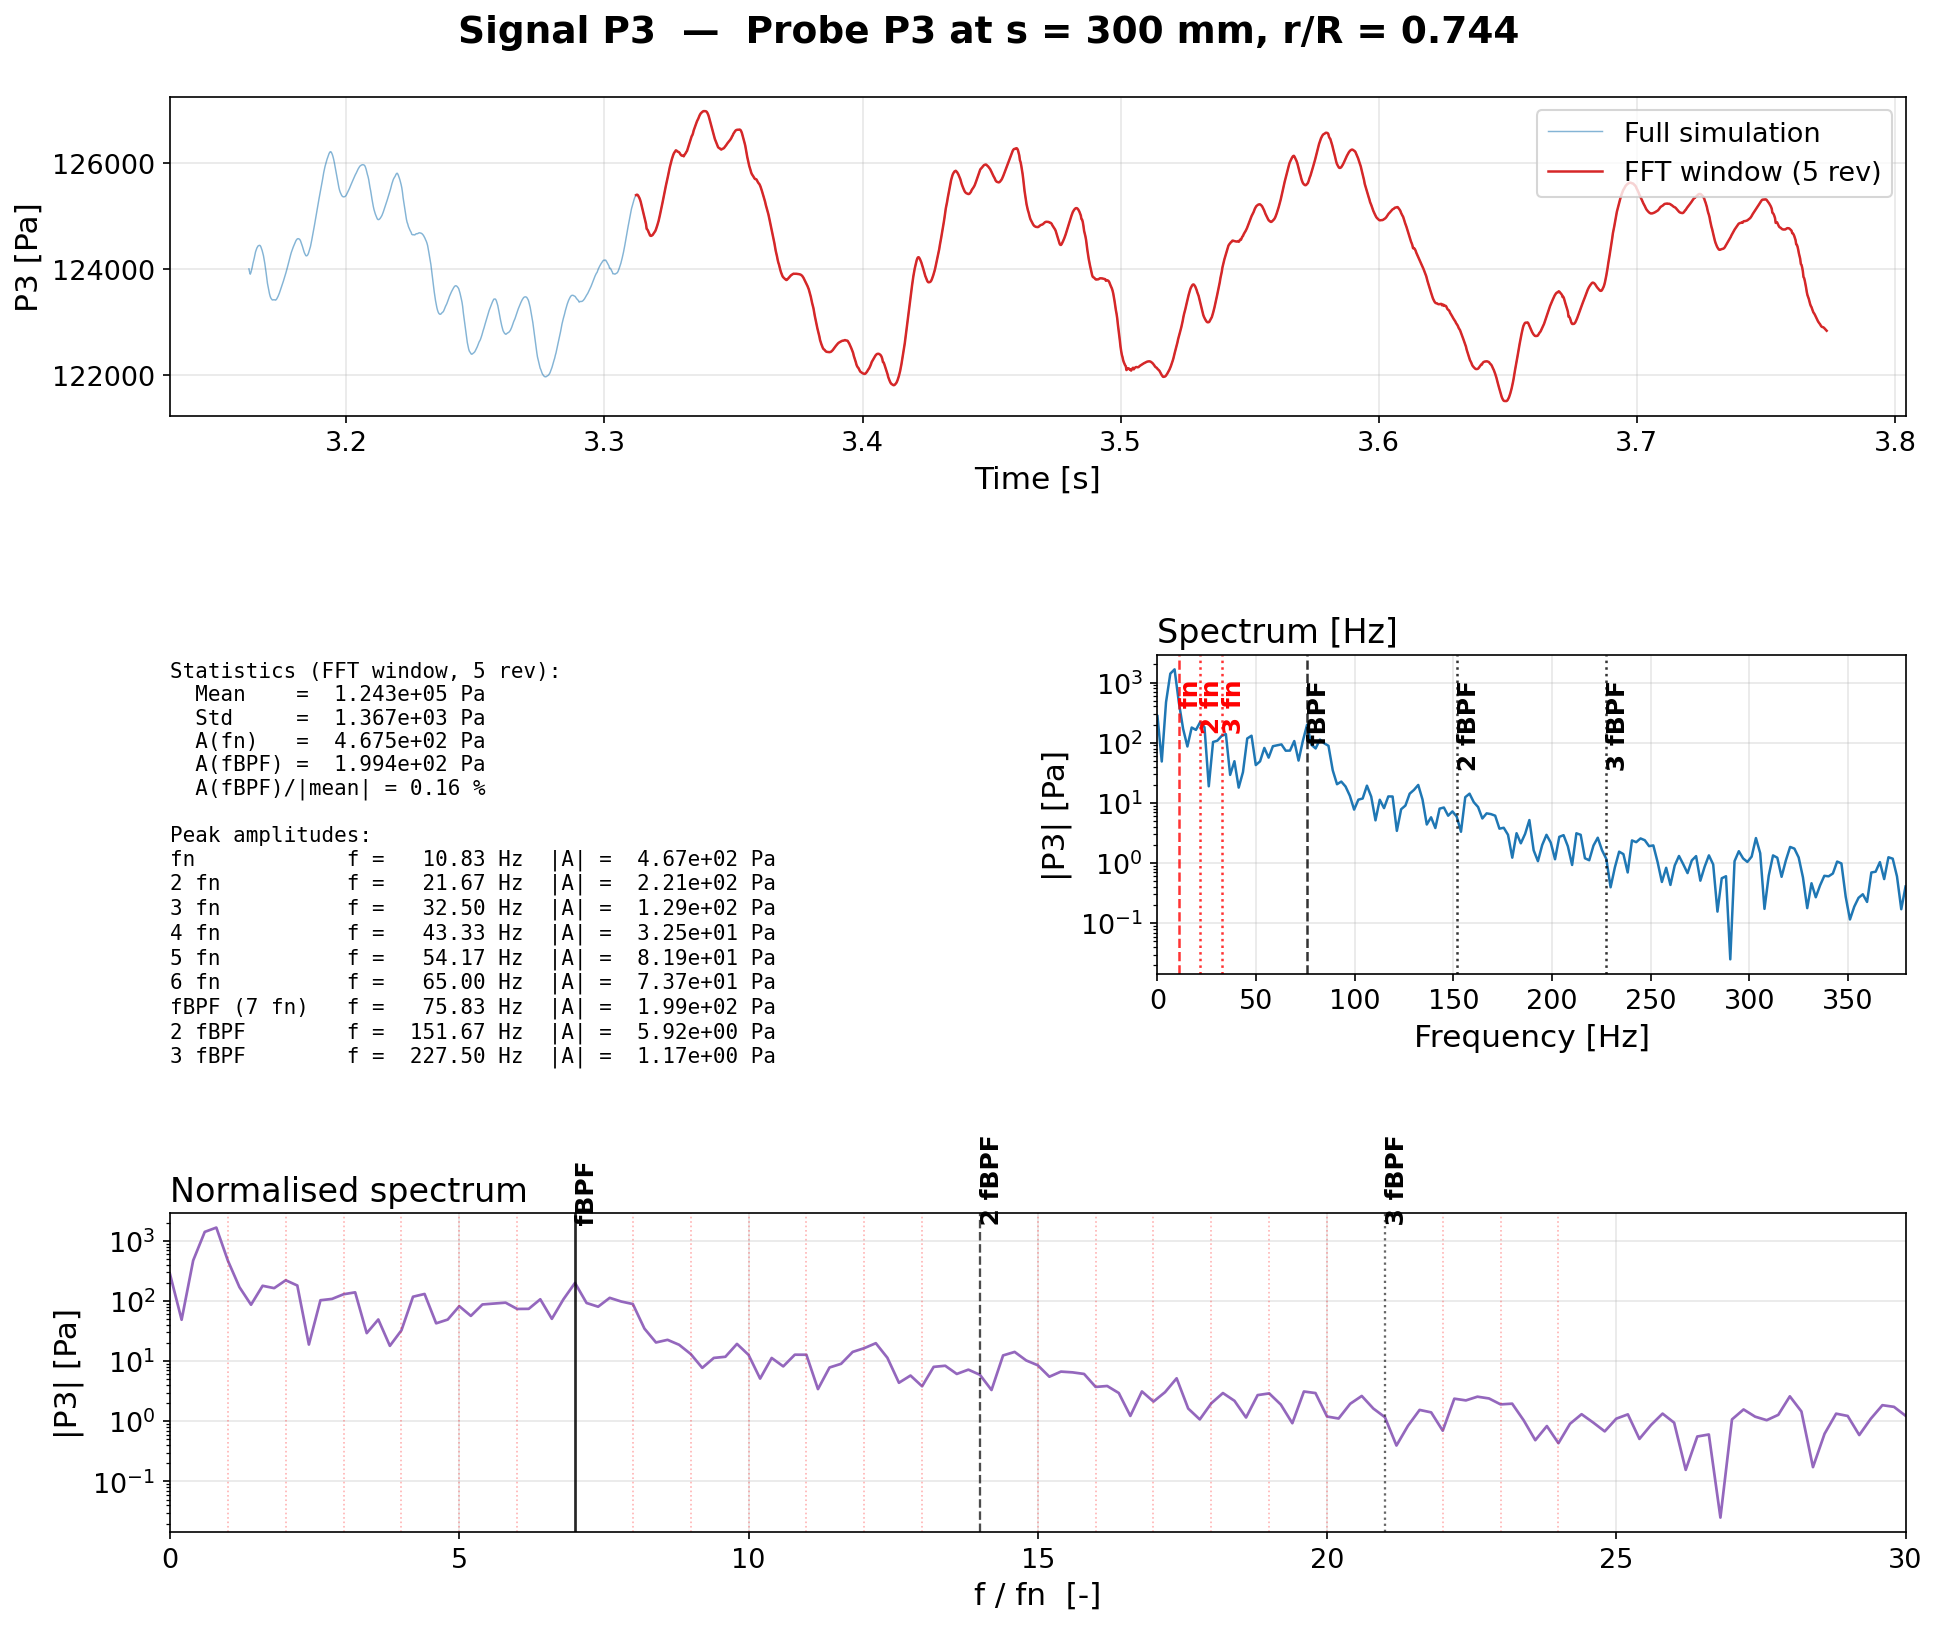
\includegraphics[width=0.99\linewidth]{Figures/FFT/signal_P3.png}
\caption{$P_3$ — Wall probe at $s = 300$~mm, $r/R = 0.744$.}
\end{figure}

\begin{figure}[H]\centering
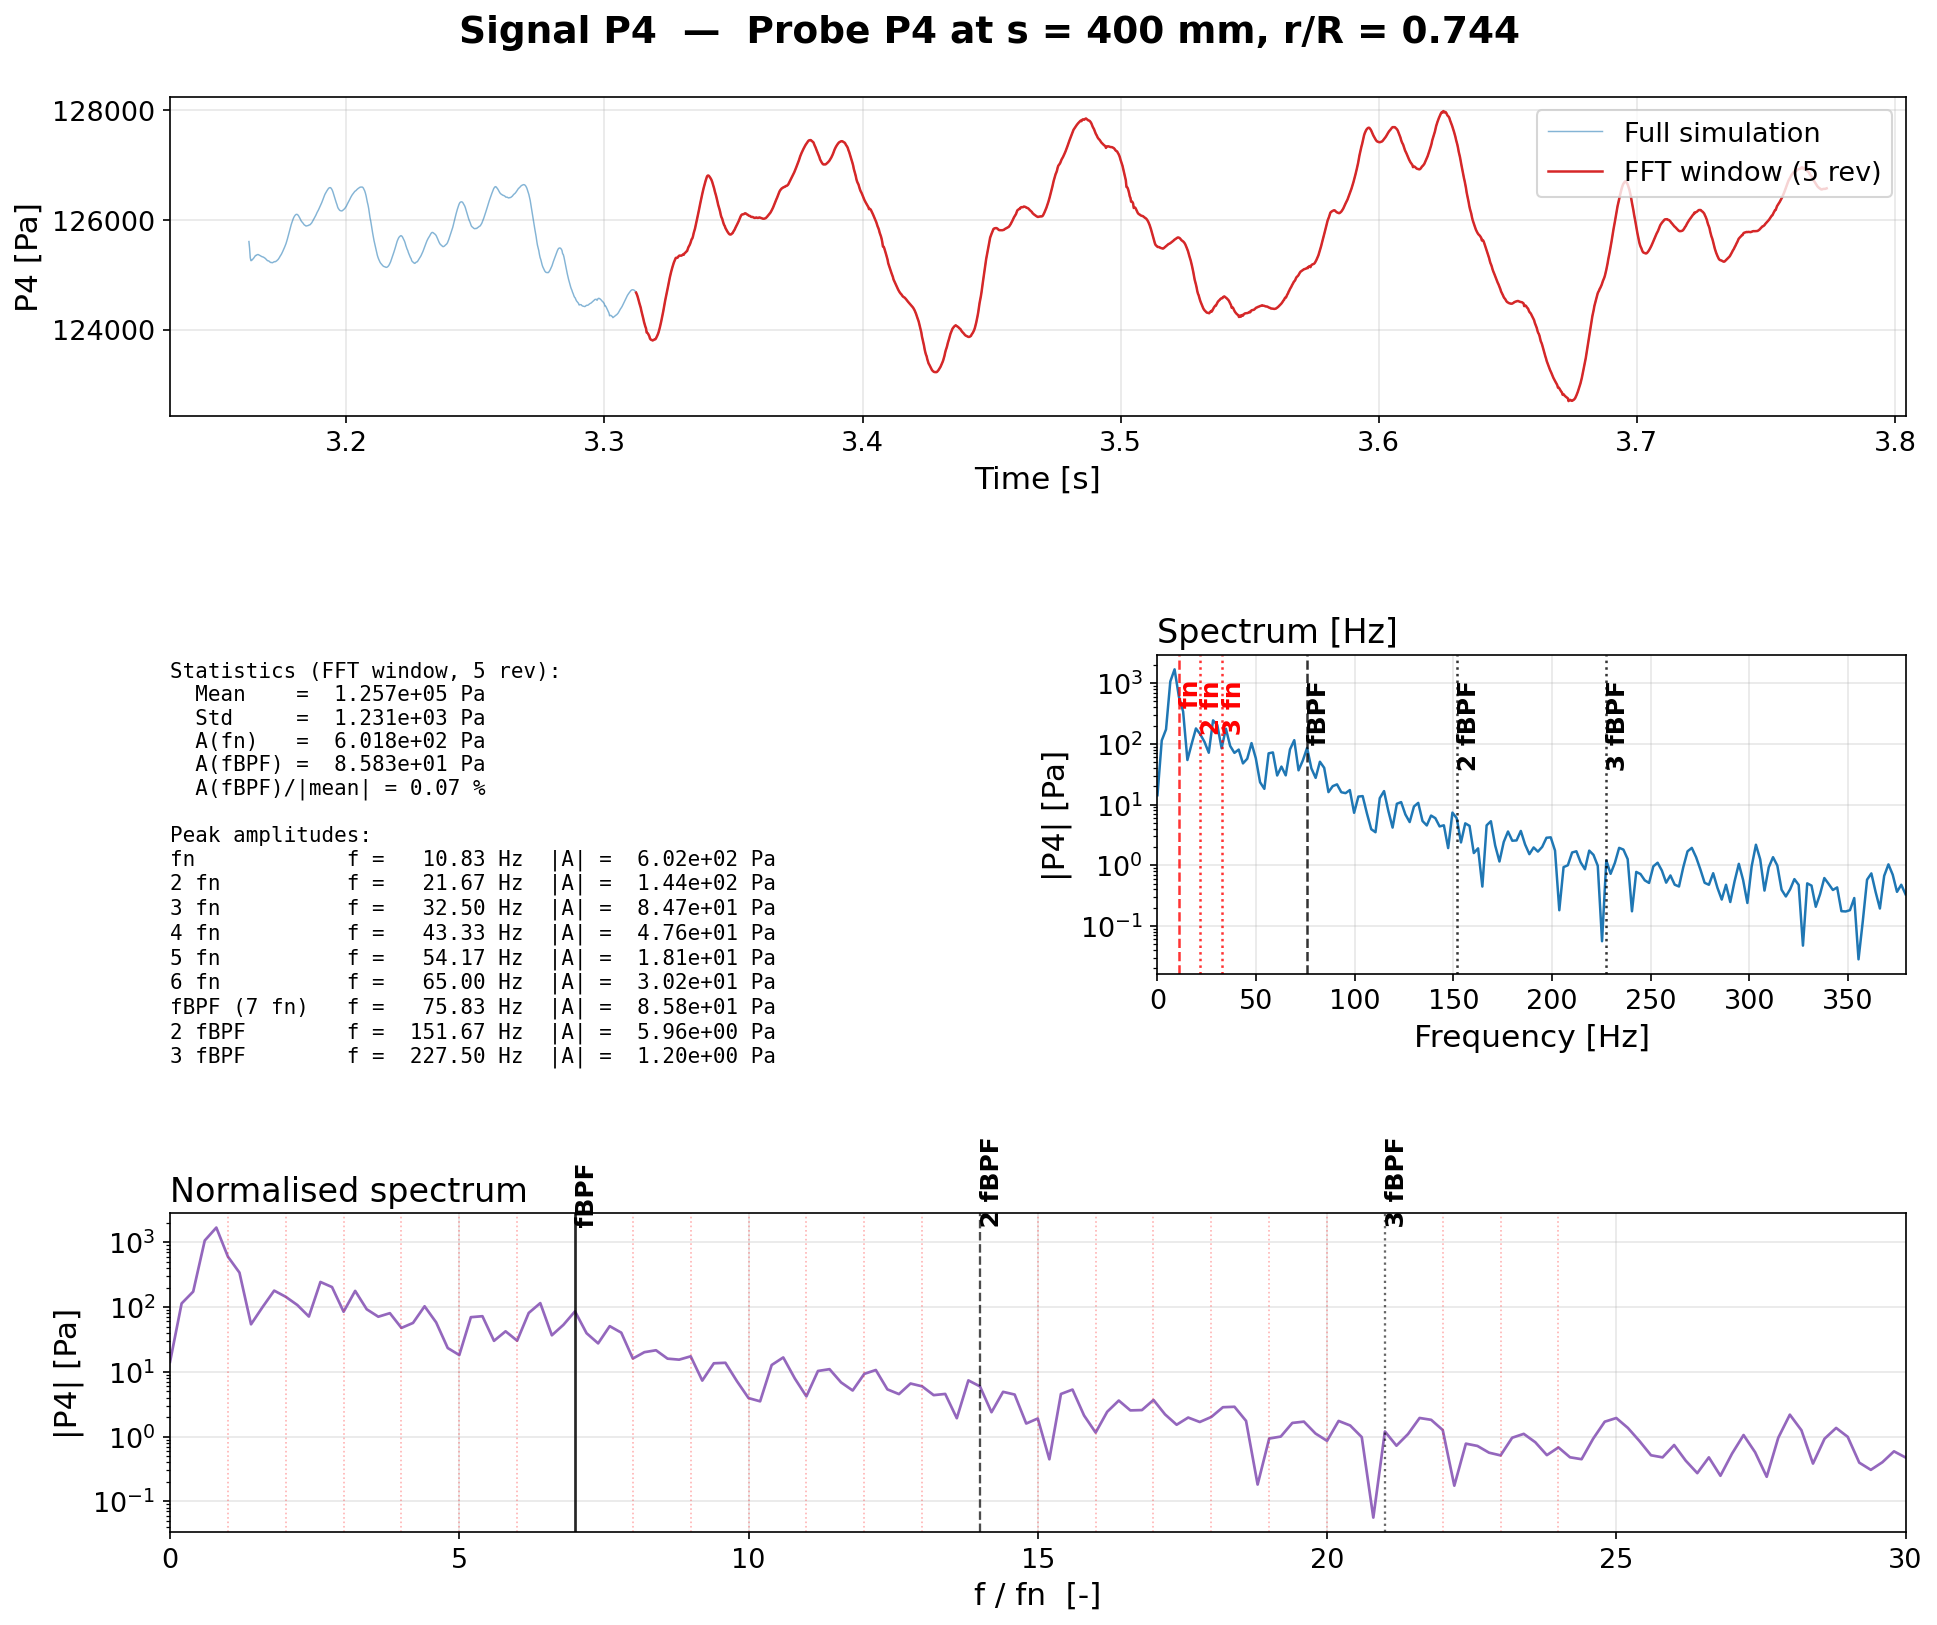
\includegraphics[width=0.99\linewidth]{Figures/FFT/signal_P4.png}
\caption{$P_4$ — Wall probe at $s = 400$~mm, $r/R = 0.744$.}
\end{figure}

\begin{figure}[H]\centering
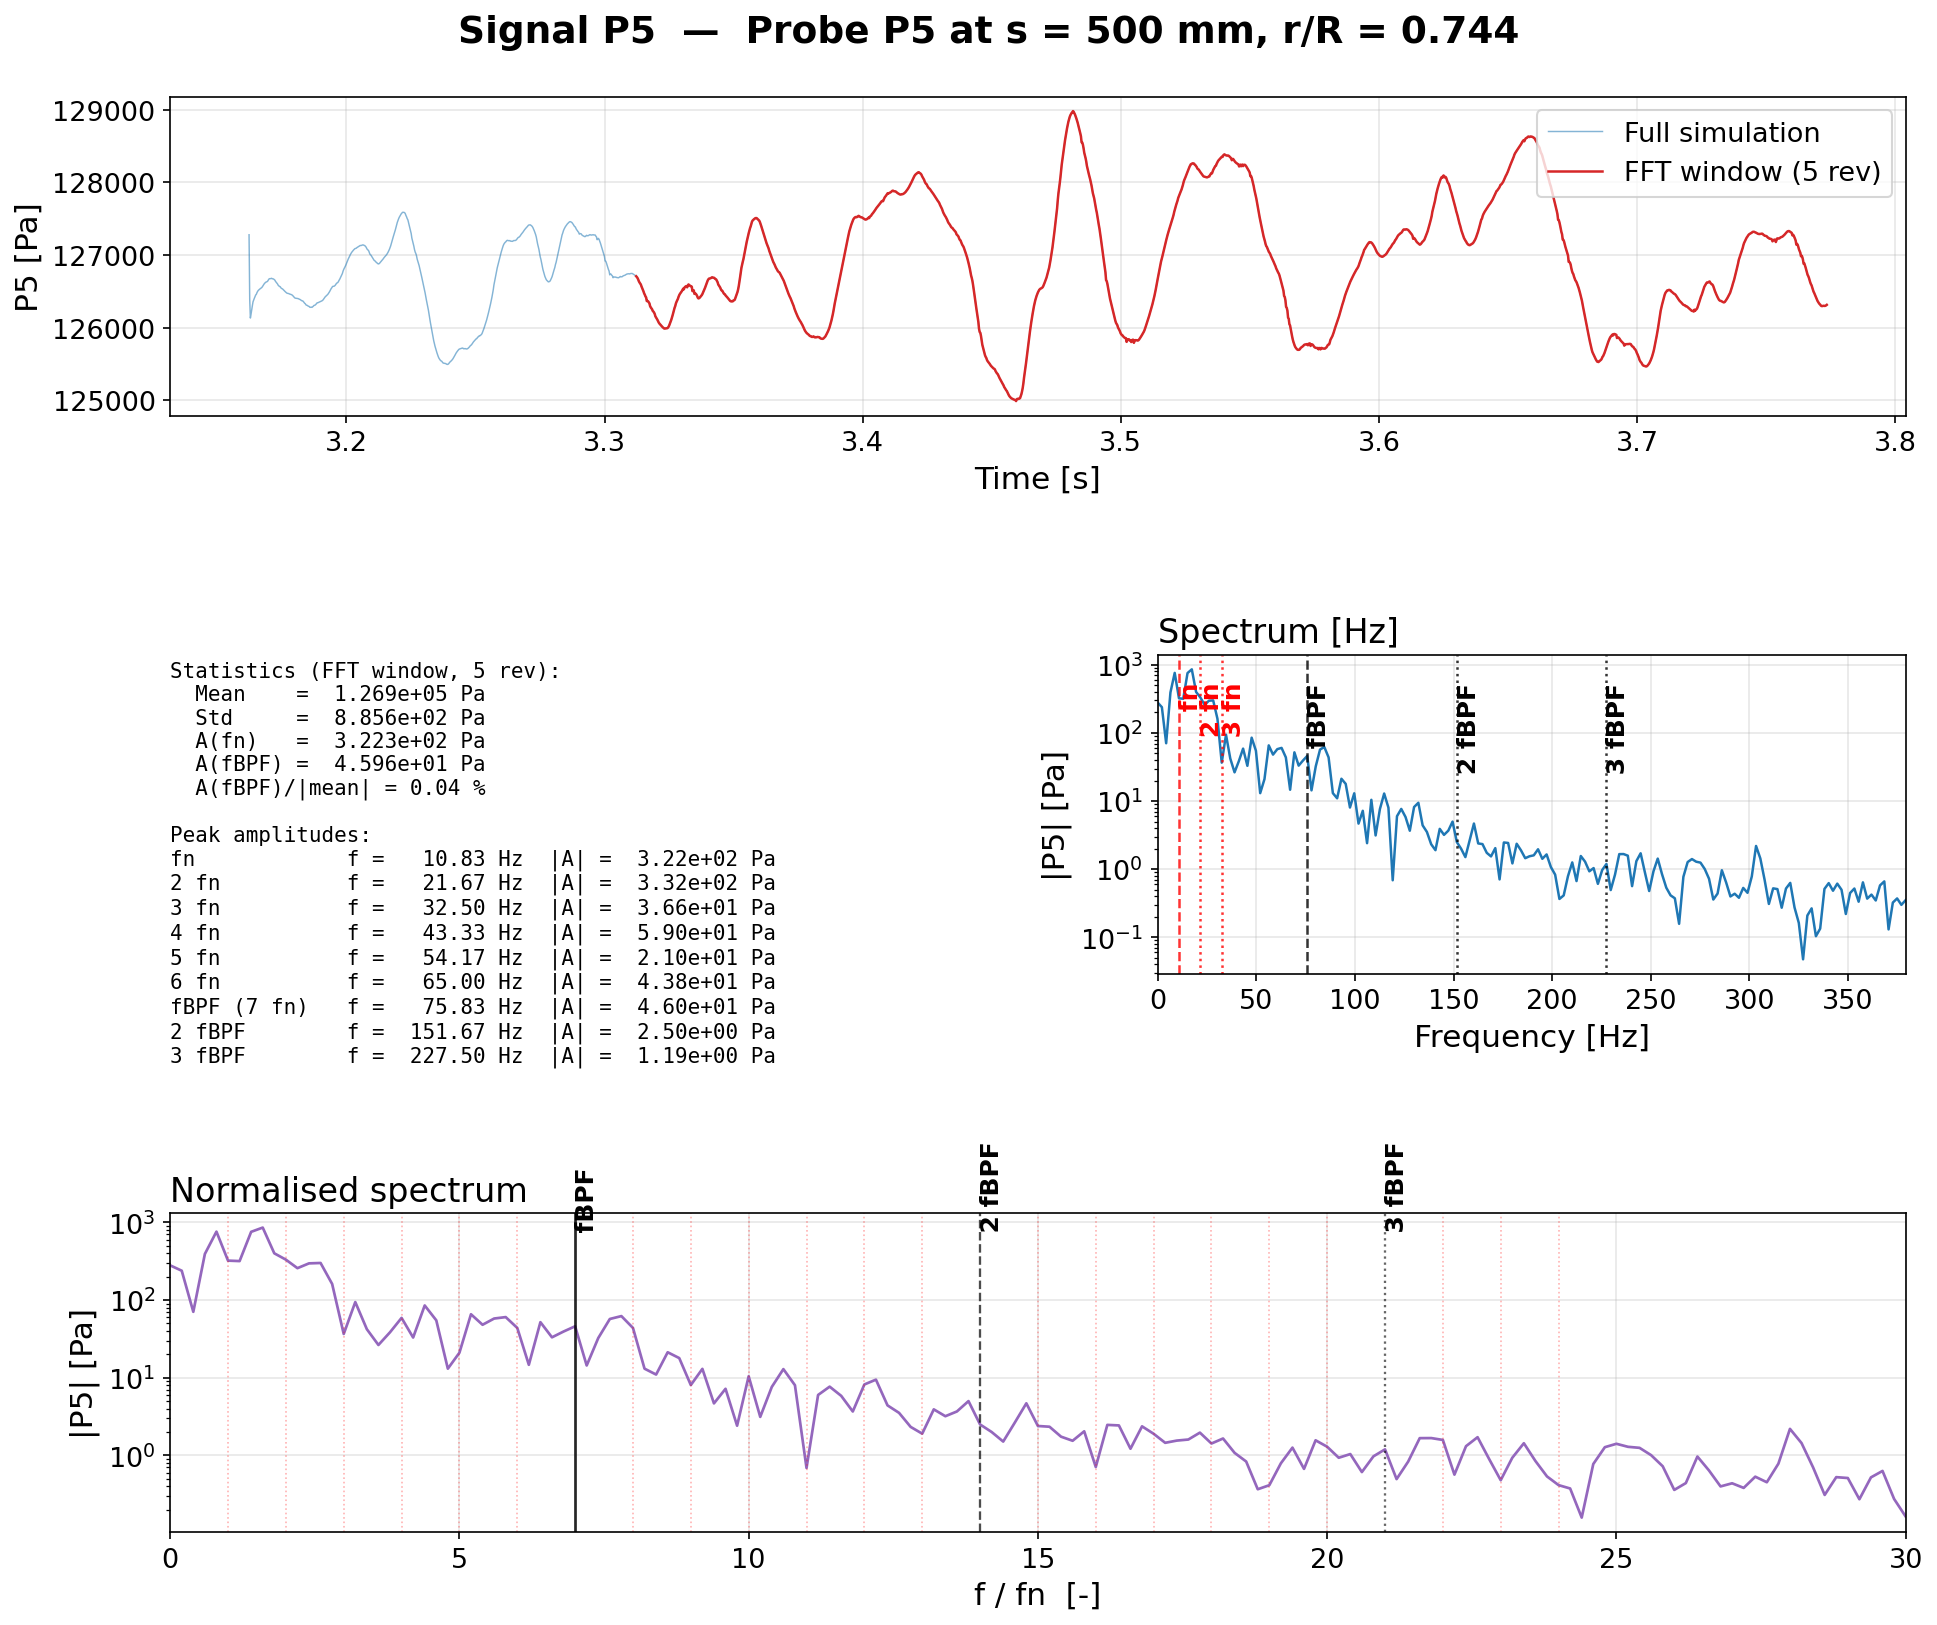
\includegraphics[width=0.99\linewidth]{Figures/FFT/signal_P5.png}
\caption{$P_5$ — Wall probe at $s = 500$~mm, $r/R = 0.744$.}
\end{figure}

\clearpage % Keep this at the end of the chapter